\documentclass[12pt]{beamer}
\usefonttheme{default}
\usetheme{Szeged}
\usecolortheme{dolphin}

\setbeamertemplate{navigation symbols}{}
\usepackage[utf8]{inputenc}
\usepackage{graphicx}
\usepackage{subcaption}
\usepackage{tikz}
\graphicspath{ {./images/} }
\usepackage{hyperref}
\usepackage{array}
\usepackage{xcolor}
\usepackage{hyperref}
\usepackage{orcidlink}
\usepackage{todonotes}
\usepackage{tabularx}
\usepackage[spanish]{babel} % Paquete para idioma español
\usepackage{caption}
\hypersetup{
  colorlinks=true,
  linkcolor=black,
  urlcolor=blue
}
\usepackage[
backend=biber,
style=ieee,
]{biblatex}
\addbibresource{references.bib}
\setbeamercolor{title}{fg=black}

%%%%%%%%%%%%%%%%%%%%%%%%%%%%%%%%%%%%%%%
%%%%% General data information %%%%% 
%%%%%%%%%%%%%%%%%%%%%%%%%%%%%%%%%%%%%%%
  \newcommand{\AutorName}{Josué Romeo Aldana Aguilar}
  \newcommand{\Grade}{Ing. Eléctrica}
  \newcommand{\Titule}{Diseño y Simulación de un Sistema de  \\ Energía Basado en COTS para \\Globos de Gran Altitud}
  \title[Electrical Power System (EPS)]{\Titule}
  \author{\textbf{\orcidlink{0000-0002-7686-5065}~\AutorName}}

  \subtitle{Tesis de grado}
  \institute[\text{Universidad Don Bosco}]{Escuela de Ingeniería Eléctrica\\
  Universidad Don Bosco \\
  El Salvador}
  \date[CEC 2023]{\\ Enero 2024}

  % Redefine el comando caption para eliminar el prefijo "Figura" y añadir "Fig. X:"
  \captionsetup[figure]{labelformat=empty,labelsep=none}
  \newcommand{\mycaption}[1]{\caption{\textbf{Fig. \thefigure:} #1}}

  \captionsetup[table]{
    labelfont=bf,
    labelsep=newline,
    justification=centering,
    textfont=it,
    name=Tabla
  }

  \begin{document}

  %------------ PORTADA -----------------

%*Inserto los logos de la UDB
\newlength{\mylogoheight}
\setlength{\mylogoheight}{2cm}
\logo{
    \hspace{0.5cm}% Espacio desde el borde izquierdo
    
\includegraphics[height=0.75\mylogoheight]{images/logo_UDB.png}
    \hspace{\dimexpr\paperwidth-2.5cm-1.5\mylogoheight}% Ajusta el espacio para el segundo logo
    
\includegraphics[height=0.75\mylogoheight]{omm_logo.png}
    \hspace{0.25cm}% Espacio al final, para balancear
}
\frame{\titlepage}
%------------ PORTADA -----------------


%--------- TABLA DE CONTENIDOS --------

%*Quito el logo de la UDB
\setlength{\mylogoheight}{0cm} 
\logo{
\includegraphics[height=\mylogoheight]{images/omm_logo.png}}
%*Quito el logo de la UDB


\begin{frame}
  \begin{tikzpicture}[remember picture, overlay]
    % Posiciona la imagen en la parte inferior del frame
    \node[opacity=0.19, anchor=south] at (current page.south) {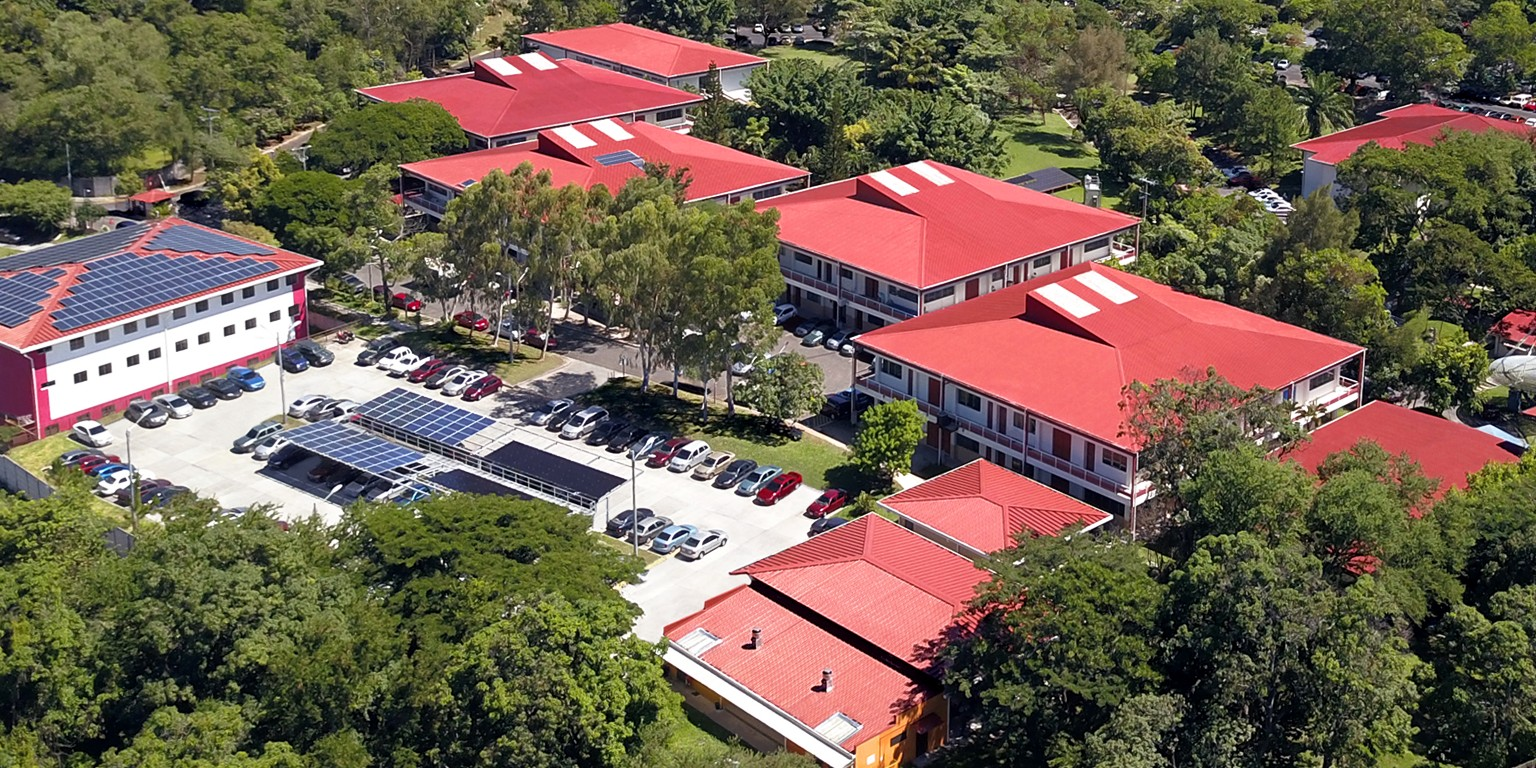
\includegraphics[width=\paperwidth,height=0.89\paperheight]{images/CampusUDB.jpg}};
  \end{tikzpicture}
  \frametitle{Tabla de Contenidos}
  \setbeamerfont{section in toc}{series=\bfseries}
  \tableofcontents
\end{frame}


%--------- TABLA DE CONTENIDOS --------


%--------- CUERPO DE LA PRESENTACION --------

\section{Introducción}
\input{Introducción}
\newpage

\section{Requerimientos}
%PAGINA 1

\begin{frame}
    \frametitle{Trayectoria de un HAB}
    Para analizar la trayectoria, empleamos el software de la Universidad de Cambridge, CUSF, que proporciona datos detallados de latitud, longitud y altitud con marcas de tiempo minuto a minuto (ver Fig. \ref{fig:ruta}).    
    \begin{figure}[H]
        \centering
        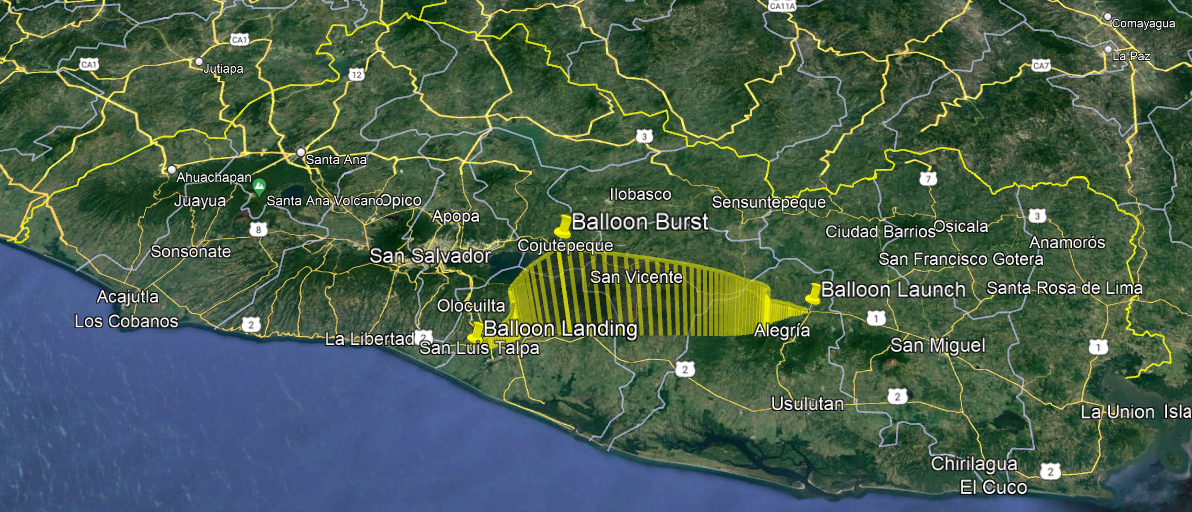
\includegraphics[width=0.75\textwidth]{ruta.png} % Ajusta el tamaño según sea necesario
        \mycaption{Simulación de Trayectoria}
        \label{fig:ruta}
    \end{figure}
    
\end{frame}

%PAGINA 2

\begin{frame}
    \frametitle{Condiciones Ambientales}

Integrando el estándar ISA con datos del CUSF mejora el análisis de variables como temperatura y presión, permitiendo predecir valores límite y tasas de cambio (ver Fig. \ref{fig:enviromentalV}).
      \begin{figure}[H]
        \centering
        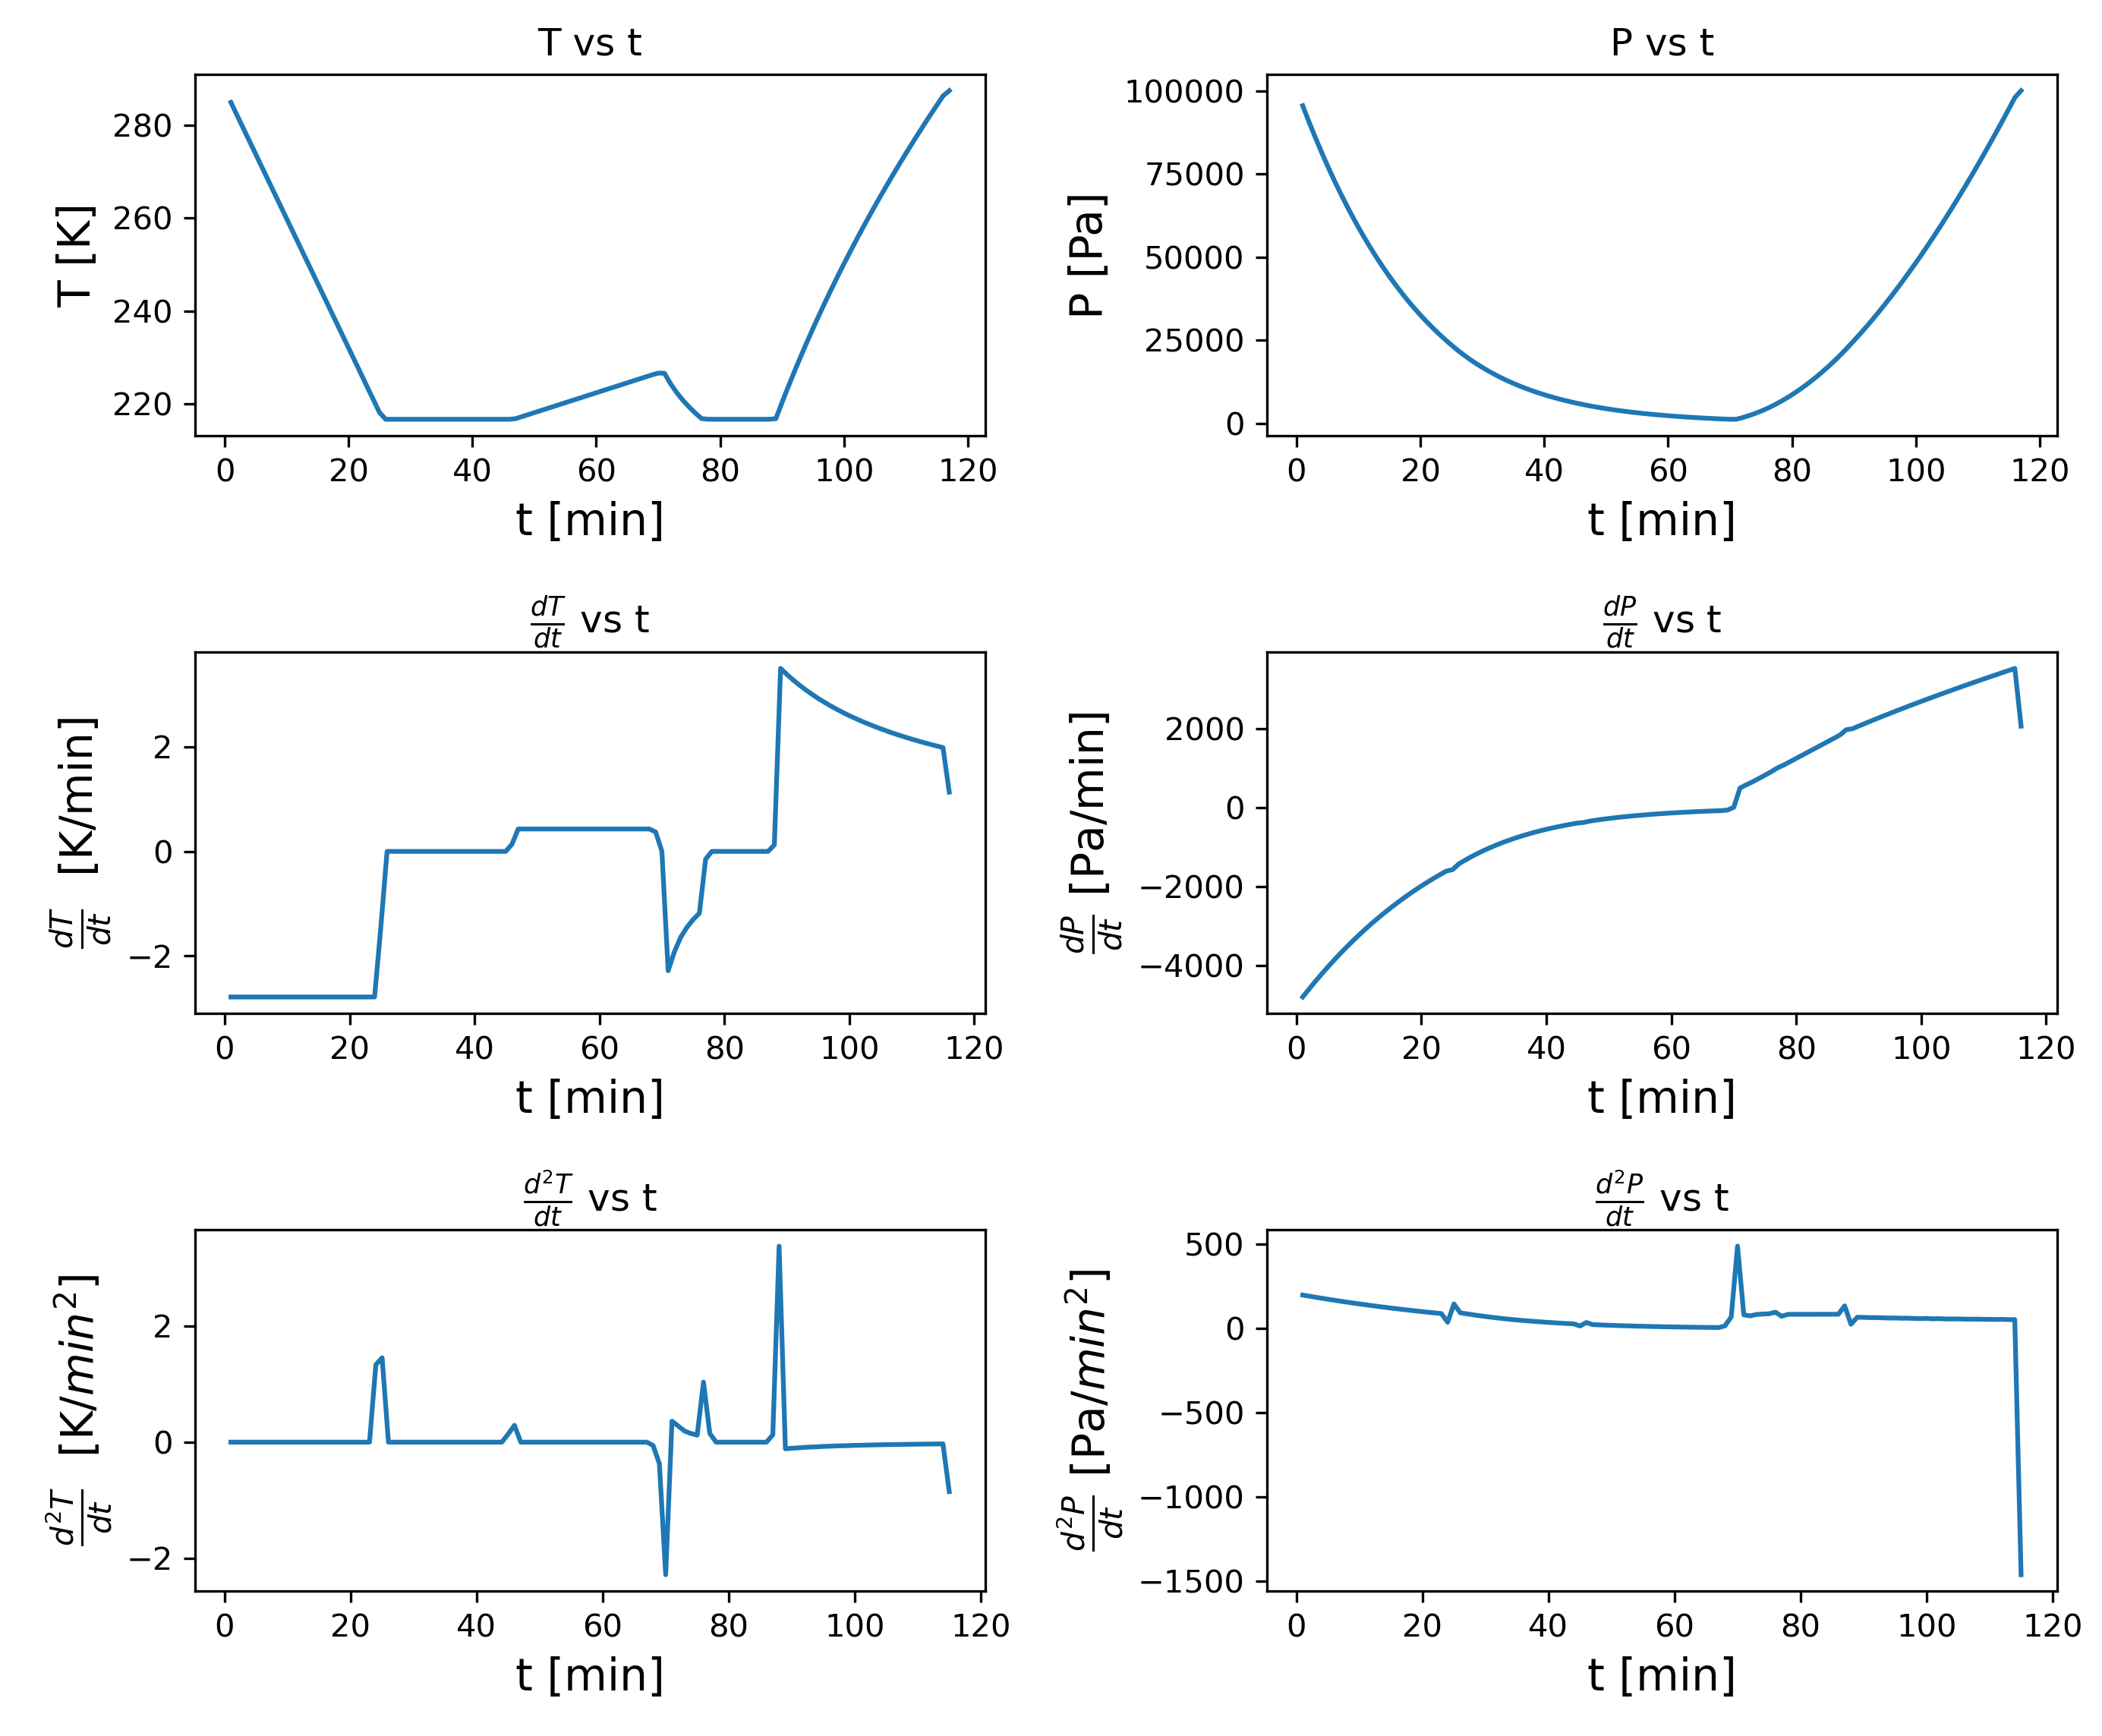
\includegraphics[width=0.75\textwidth]{EnviromentalVariables.png} % Ajusta el tamaño según sea necesario
        \mycaption{Variables atmosféricas en trayectoria de HAB}
        \label{fig:enviromentalV}
    \end{figure}
    
\end{frame}

% PAGINA 3


\begin{frame}
\frametitle{Condiciones Ambientales}

Las condiciones extremas en la estratósfera pueden alcanzar -56.50\textdegree{}C y 1.20\% de la presión atmosférica estándar. Se observaron razones de cambio máximas de -2.78\textdegree{}C por minuto y una pérdida de presión atmosférica del 4.74\% por minuto.\\ 
\vspace*{0.5 cm}
Estudios como el experimento TASEC-Lab \cite{TASEC} no solo validan estos datos, sino que también identifican una franja crítica alrededor de los 11 km de altitud, cerca de la tropopausa, con notables variaciones térmicas, un aspecto crucial para la selección de componentes y sistemas de control térmico.

   
\end{frame}



% PAGINA 4

\begin{frame}
\frametitle{Presupuesto Energético}

\begin{table}[!ht]
    \centering
    \caption{Cuadro de cargas para bus 3.3v}
    \label{tab:cuadro-cargas1}
    \resizebox{\columnwidth}{!}{% Escala la tabla para que se ajuste al ancho de la columna
    \begin{tabular}{llllllll}
    \hline
    \textbf{Descripción} & \textbf{Cantidad} & \textbf{Subsistema} & \textbf{I [mA]} & \textbf{P [W]} & \textbf{t [h]} & \textbf{E [Wh]} & \textbf{Q [mAh]} \\
    \hline
    MCU 1 & 1 unidad & Telemetría & 93.00 & 0.31 & 6.00 & 1.84 & 558 \\ 
    LoRa & 1 unidad & Telemetría & 630.00 & 2.08 & 6.00 & 12.47 & 3780 \\ 
    MCU 2 & 1 unidad & Navegación & 61.00 & 0.20 & 6.00 & 1.21 & 366.00 \\ 
    GNSS & 1 unidad & Navegación & 100.00 & 0.33 & 6.00 & 1.98 & 600.00 \\ 
    RTD & 1 unidad & Navegación & 3.50 & 0.01 & 6.00 & 0.07 & 21.00 \\ 
    IMU & 1 unidad & Navegación & 0.60 & 0.00 & 6.00 & 0.01 & 3.60 \\ 
    MCU 3 & 1 unidad & Carga útil & 70.00 & 0.23 & 2.00 & 0.46 & 140.00 \\ 
    Cámara IR & 1 unidad & Carga útil & 25.00 & 0.08 & 2.00 & 0.17 & 50.00 \\
    \hline
    & & \textbf{I Total} & 983.10 & & & & 5518.6 \\ 
    \hline
    \end{tabular}}
\end{table}

\end{frame}



% PAGINA 5

\begin{frame}
    \frametitle{Presupuesto Energético}
    
    \begin{table}[!ht]
        \centering
        \caption{Cuadro de cargas para bus 5.0v}
        \label{tab:cuadro-cargas2}
        \resizebox{\columnwidth}{!}{% Escala la tabla para que se ajuste al ancho de la columna
        \begin{tabular}{llllllll}
            \hline
            \textbf{Descripción} & \textbf{Cantidad} & \textbf{Subsistema} & \textbf{I [mA]} & \textbf{P [W]} & \textbf{t [h]} & \textbf{E [Wh]} & \textbf{Q [mAh]} \\
            \hline
            RTC & 1 unidad & Navegación & 0.30 & 0.00 & 6.00 & 0.01 & 1.80 \\
            Buzzer & 1 unidad & Navegación & 24.00 & 0.12 & 6.00 & 0.72 & 144 \\
            Barómetro & 1 unidad & Navegación & 0.00 & 0.00 & 6.00 & 0.00 & 0.00 \\
            MUX & 1 unidad & Navegación & 100.00 & 0.50 & 6.00 & 3.00 & 600 \\
            Datalogger 1 & 1 unidad & Navegación & 6.00 & 0.03 & 6.00 & 0.18 & 36 \\
            Cámara & 1 unidad & Carga útil & 260.00 & 1.30 & 2.00 & 2.60 & 520 \\
            Datalogger 2 & 1 unidad & Carga útil & 12.00 & 0.06 & 2.00 & 0.12 & 24 \\
            \hline
            ~ & ~ & \textbf{I Total} & 402.30 & ~ & ~ & ~ & 1325.8 \\
            \hline
        \end{tabular}}
    \end{table}
    
    
    \end{frame}


% PAGINA 6

\begin{frame}
    \frametitle{Limitaciones en Masa y Volumen}
    En la misión \textit{StratoBalloon}, el módulo de impresión 3D destina dos niveles al EPS (Fig. \ref{fig:Estructura1}), a 2.54 cm de distancia, según la Fig. \ref{fig:Estructura2} \cite{Reyes2023}. El peso máximo para el EPS es 600 gramos.
    \begin{figure}
        \centering
        \begin{minipage}{.5\textwidth}
            \centering
            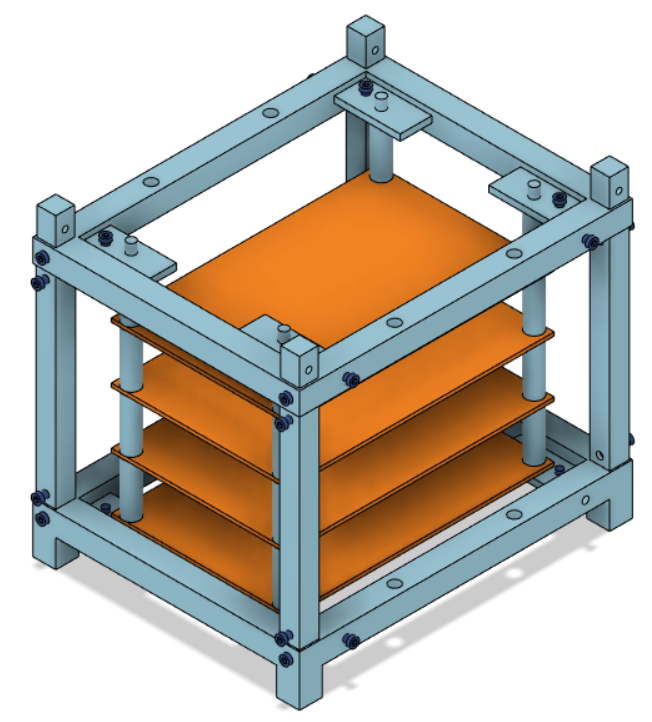
\includegraphics[width=0.48\textheight]{PlanoB.png} % Reemplaza con tu primera imagen
            \mycaption{Vista 1}
            \label{fig:Estructura1}
        \end{minipage}\hfill
        \begin{minipage}{.5\textwidth}
            \centering
            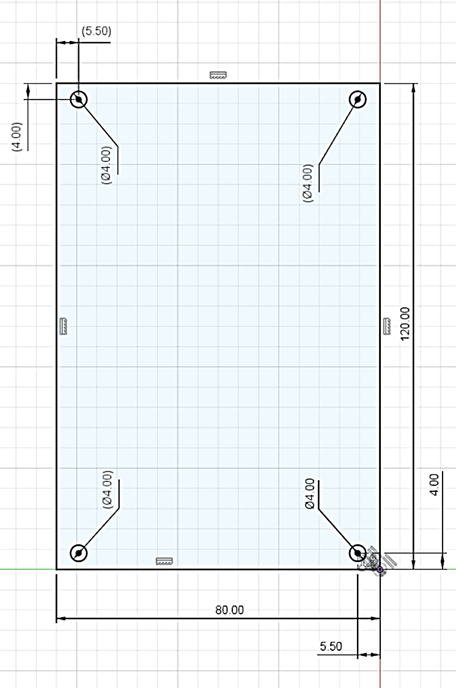
\includegraphics[width=0.45\textheight, angle=90]{PCBEspacio.png} % Reemplaza con tu segunda imagen
            \vspace*{0.25 cm}
            \mycaption{Vista 2}
            \label{fig:Estructura2}
        \end{minipage}
    \end{figure}
    \end{frame}


% PAGINA 7

\begin{frame}
    \frametitle{Resumen de Requerimientos}
    \begin{table}[!ht]
        \centering
        \caption{Requerimientos del EPS - Parte 1}
        \label{tab:requerimientos-eps-p1}
        \resizebox{\columnwidth}{!}{% Escala la tabla para que se ajuste al ancho de la columna
        \begin{tabular}{l|p{4.8cm}|p{4.8cm}|p{4.8cm}}
            \hline
            \textbf{ID} & \textbf{Descripción} & \textbf{Justificación} & \textbf{Mecanismo de verificación} \\
            \hline
            R1 & Resistencia al vacío térmico, temperatura mínima de hasta -56.50°C y 1.20\% de presión atmosférica. & Resultados en simulaciones. & Ensayos en cámara de vacío térmico \\
            \hline
            R2 & El EPS debe proveer una línea de alimentación de 3.3 V $\pm$ 1\% con una corriente mínima de 983.1 mA $\pm$ 1\%. & Bus de alimentación. & Medición de V y I.\\
            \hline
            R3 & El EPS debe proveer una línea de alimentación de 5.0 V $\pm$ 1\% con una corriente mínima de 402.30 mA $\pm$ 1\% & Bus de alimentación. & Medición de V y I. \\
            \hline
        \end{tabular}}
    \end{table}
    
    
    \end{frame}

% PAGINA 8

\begin{frame}
    \frametitle{Resumen de Requerimientos}
    \begin{table}[!ht]
        \centering
        \caption{Requerimientos del EPS - Parte 2}
        \label{tab:requerimientos-eps-p2}
        \resizebox{\columnwidth}{!}{% Escala la tabla para que se ajuste al ancho de la columna
            \begin{tabular}{l|p{4.8cm}|p{4.8cm}|p{4.8cm}}
                \hline
                \textbf{ID} & \textbf{Descripción} & \textbf{Justificación} & \textbf{Mecanismo de verificación} \\
                \hline
                R4 & No debe exceder una masa de 600 g. & Limitación de masa. & Medición de masa. \\
                \hline
                R5 & 2 PCB de 12x8 cm con 2.5 cm de altura. & Limitación de espacio. & Medición de longitud.\\
                \hline
                R6 & Registro de V [v] y I [mA]. & Función deseable. & Ensayo de registro de datos. \\
                \hline
                R7 & Registro de T [\textdegree{}C] y P [atm]. & Función deseable. & Ensayo de registro de datos. \\
                \hline
                R8 & Comunicación I2C. Recepción desde Navegación de la señal de control ON/OFF de carga útil. Transmisión de SoC a telemetría. & Integración de subsistemas. & Ensayo de comunicación. \\
                \hline
            \end{tabular}
        }
    \end{table}  
    
    \end{frame}

    % PAGINA 9

    \begin{frame}
        \frametitle{Resumen de Requerimientos}
        \begin{table}[!ht]
            \centering
            \caption{Requerimientos del EPS - Parte 3}
            \label{tab:requerimientos-eps-p3}
            \resizebox{\columnwidth}{!}{% Escala la tabla para que se ajuste al ancho de la columna
                \begin{tabular}{l|p{4.8cm}|p{4.8cm}|p{4.8cm}}
                    \hline
                    \textbf{ID} & \textbf{Descripción} & \textbf{Justificación} & \textbf{Mecanismo de verificación} \\
                    \hline
                    R9 & Control ON-OFF: carga útil.& Ahorro de energía. & Ensayo de control ON-OFF. \\
                    \hline
                    R10 & Interruptor RBF (Remove before flight, retirar antes del vuelo) para encendido y apagado del EPS.& Seguridad de la Misión, útil para prevenir accidentes. & Medición de continuidad. \\
                    \hline
                    R11 & Cargador de baterías con fuente de alimentación VDC externa & Carga del banco de baterías & Medición de voltaje. \\
                    \hline
                \end{tabular}
            }
        \end{table}
        
    \end{frame}
\newpage

\section{Arquitectura}
%PAGINA 1
\begin{frame}
    \frametitle{Arquitectura del Sistema}

    \begin{figure}[H]
        \centering
        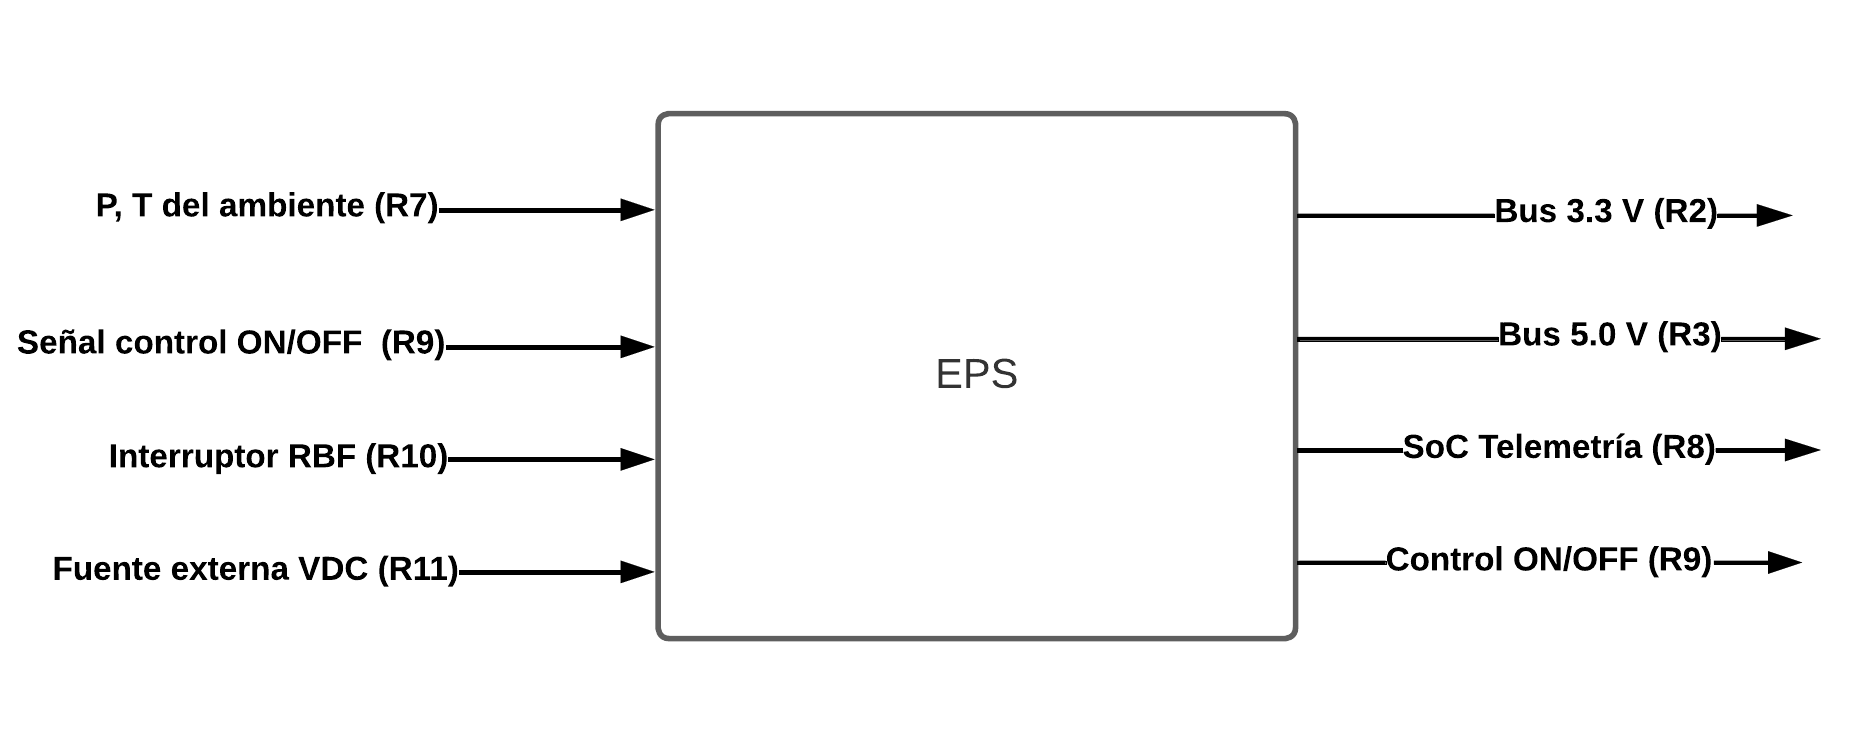
\includegraphics[width=\textwidth]{Level0.png} % Ajusta el tamaño según sea necesario
        \mycaption{Diagrama funcional nivel 0}
        \label{fig:level0DF}
    \end{figure}
\end{frame}

%PAGINA 2
\begin{frame}
    \frametitle{Arquitectura del Sistema}
    \begin{figure}[H]
        \centering
        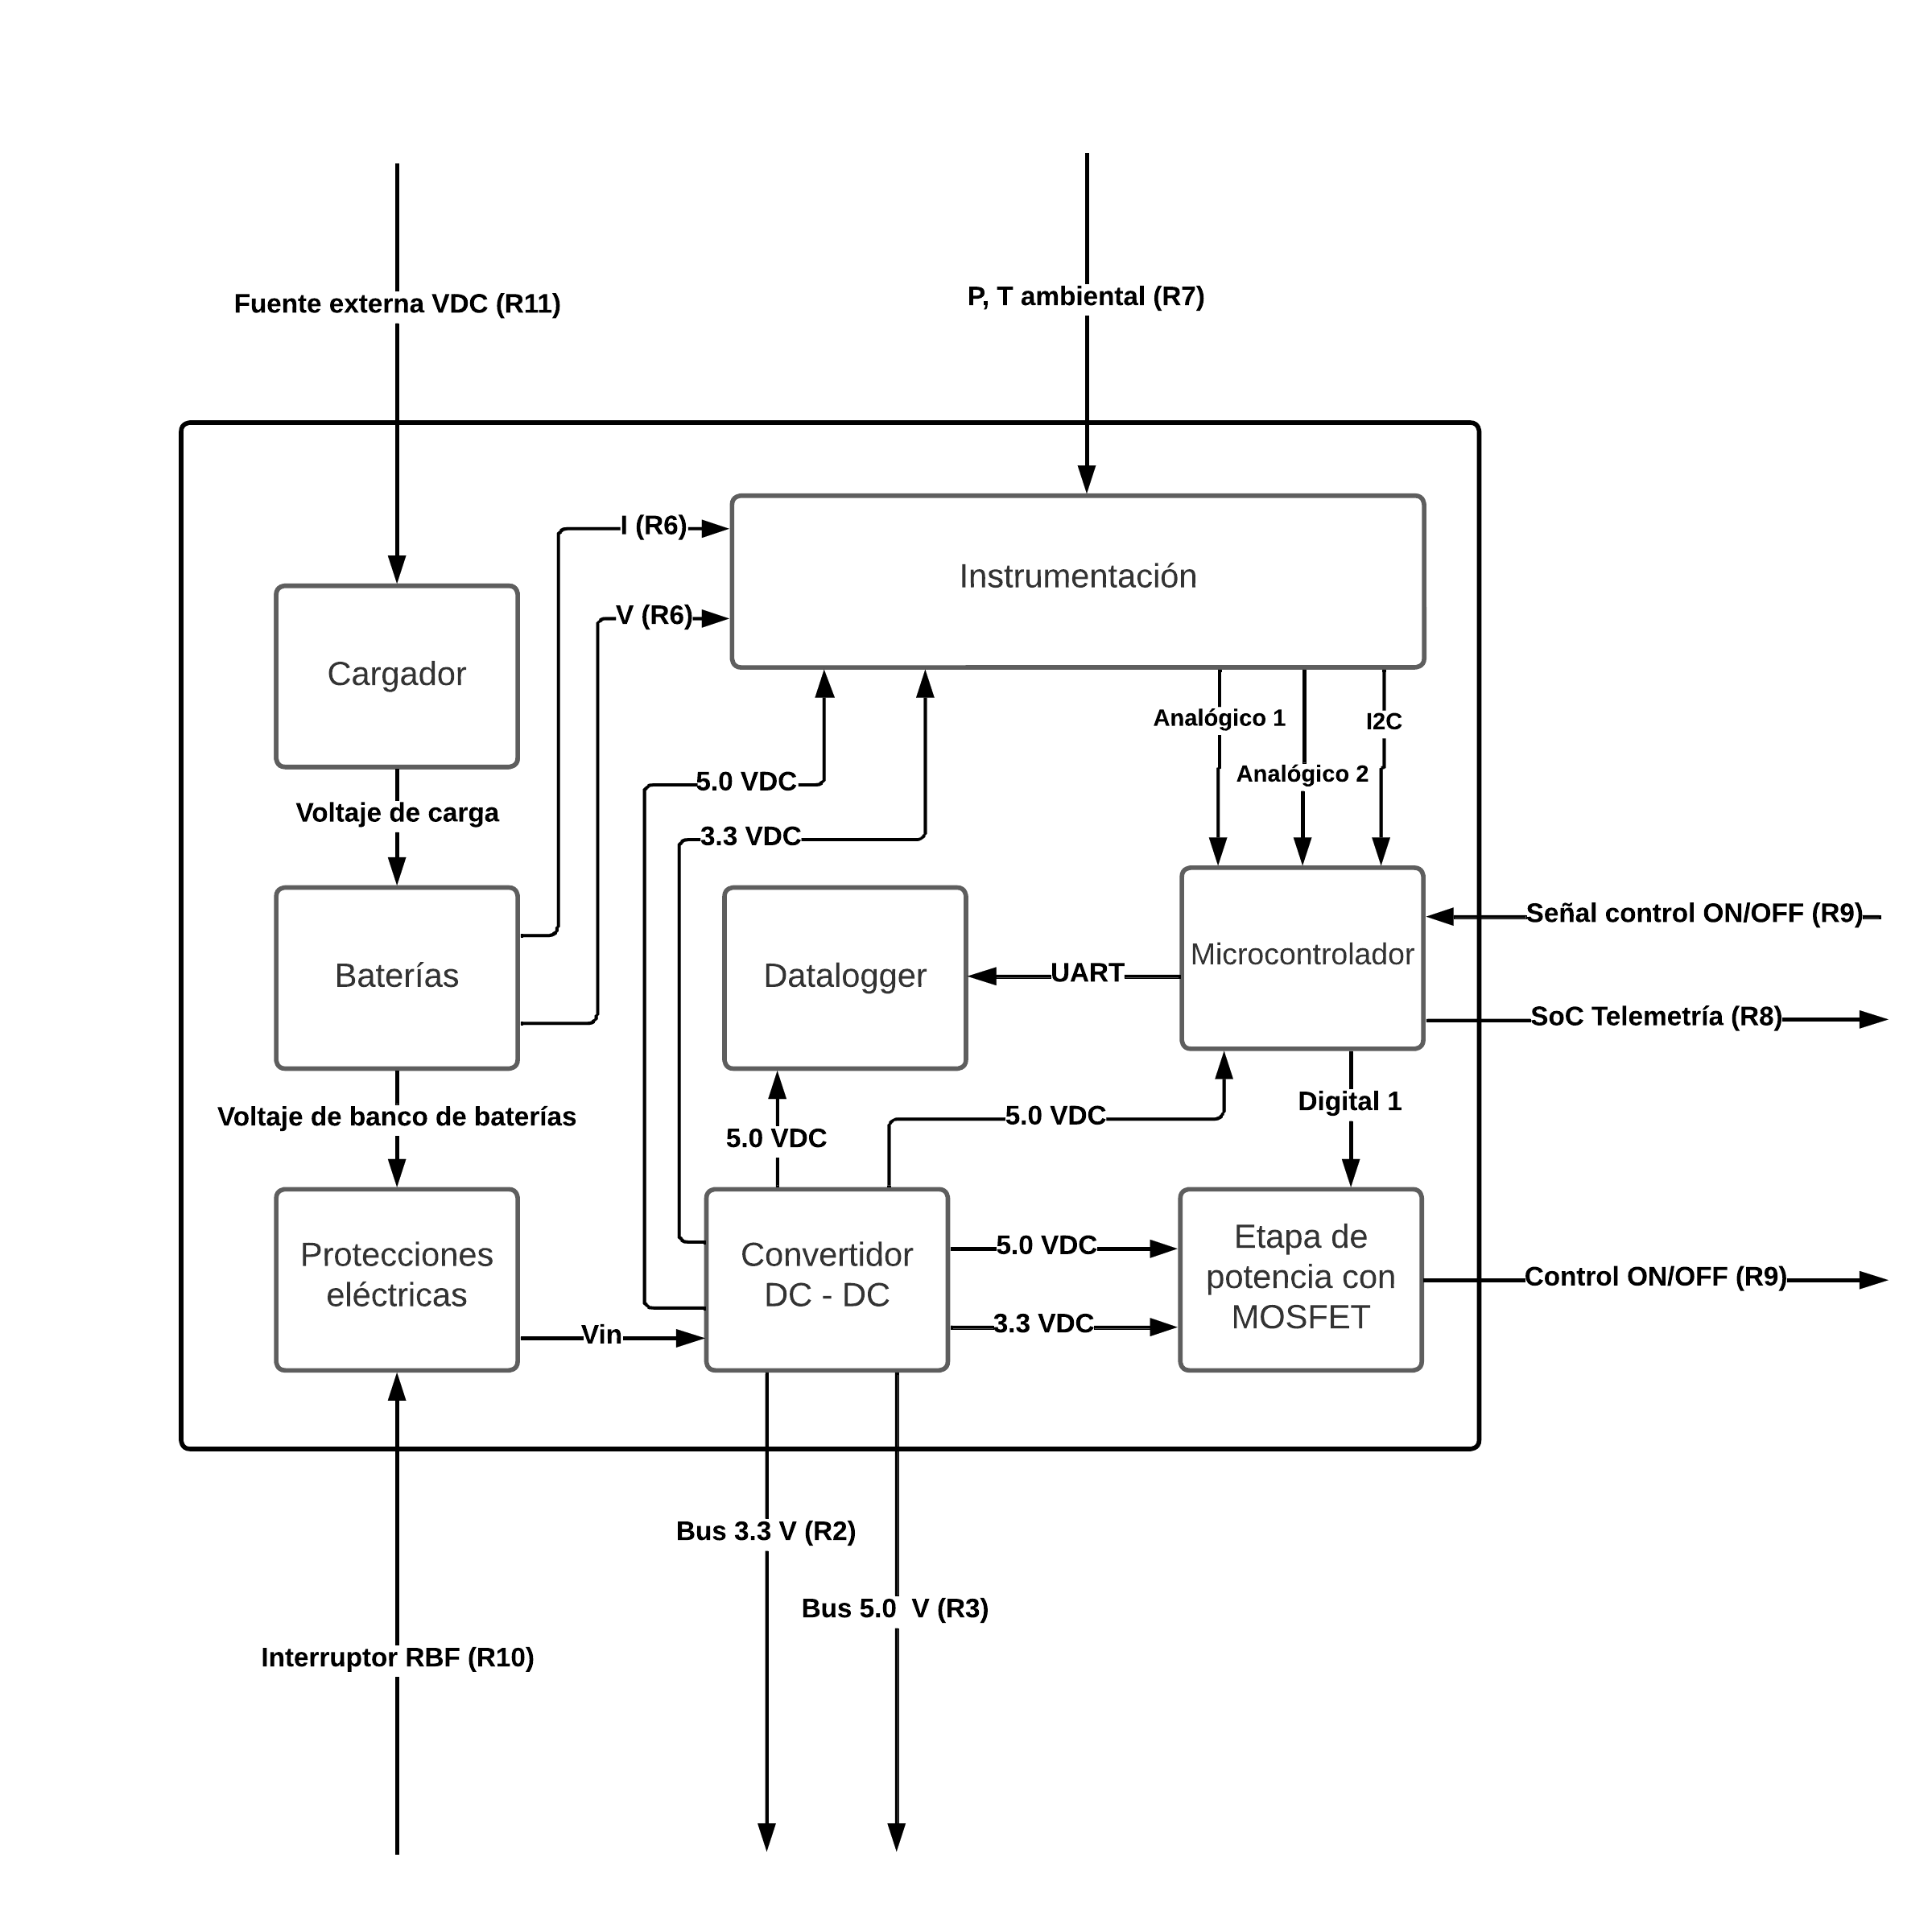
\includegraphics[width=0.60\textwidth]{Level1.png} % Ajusta el tamaño según sea necesario
        \mycaption{Diagrama funcional nivel 1}
        \label{fig:level0DF}
    \end{figure}
\end{frame}

%PAGINA 3
\begin{frame}
    \frametitle{Arquitectura del Sistema}

    \begin{figure}[H]
        \centering
        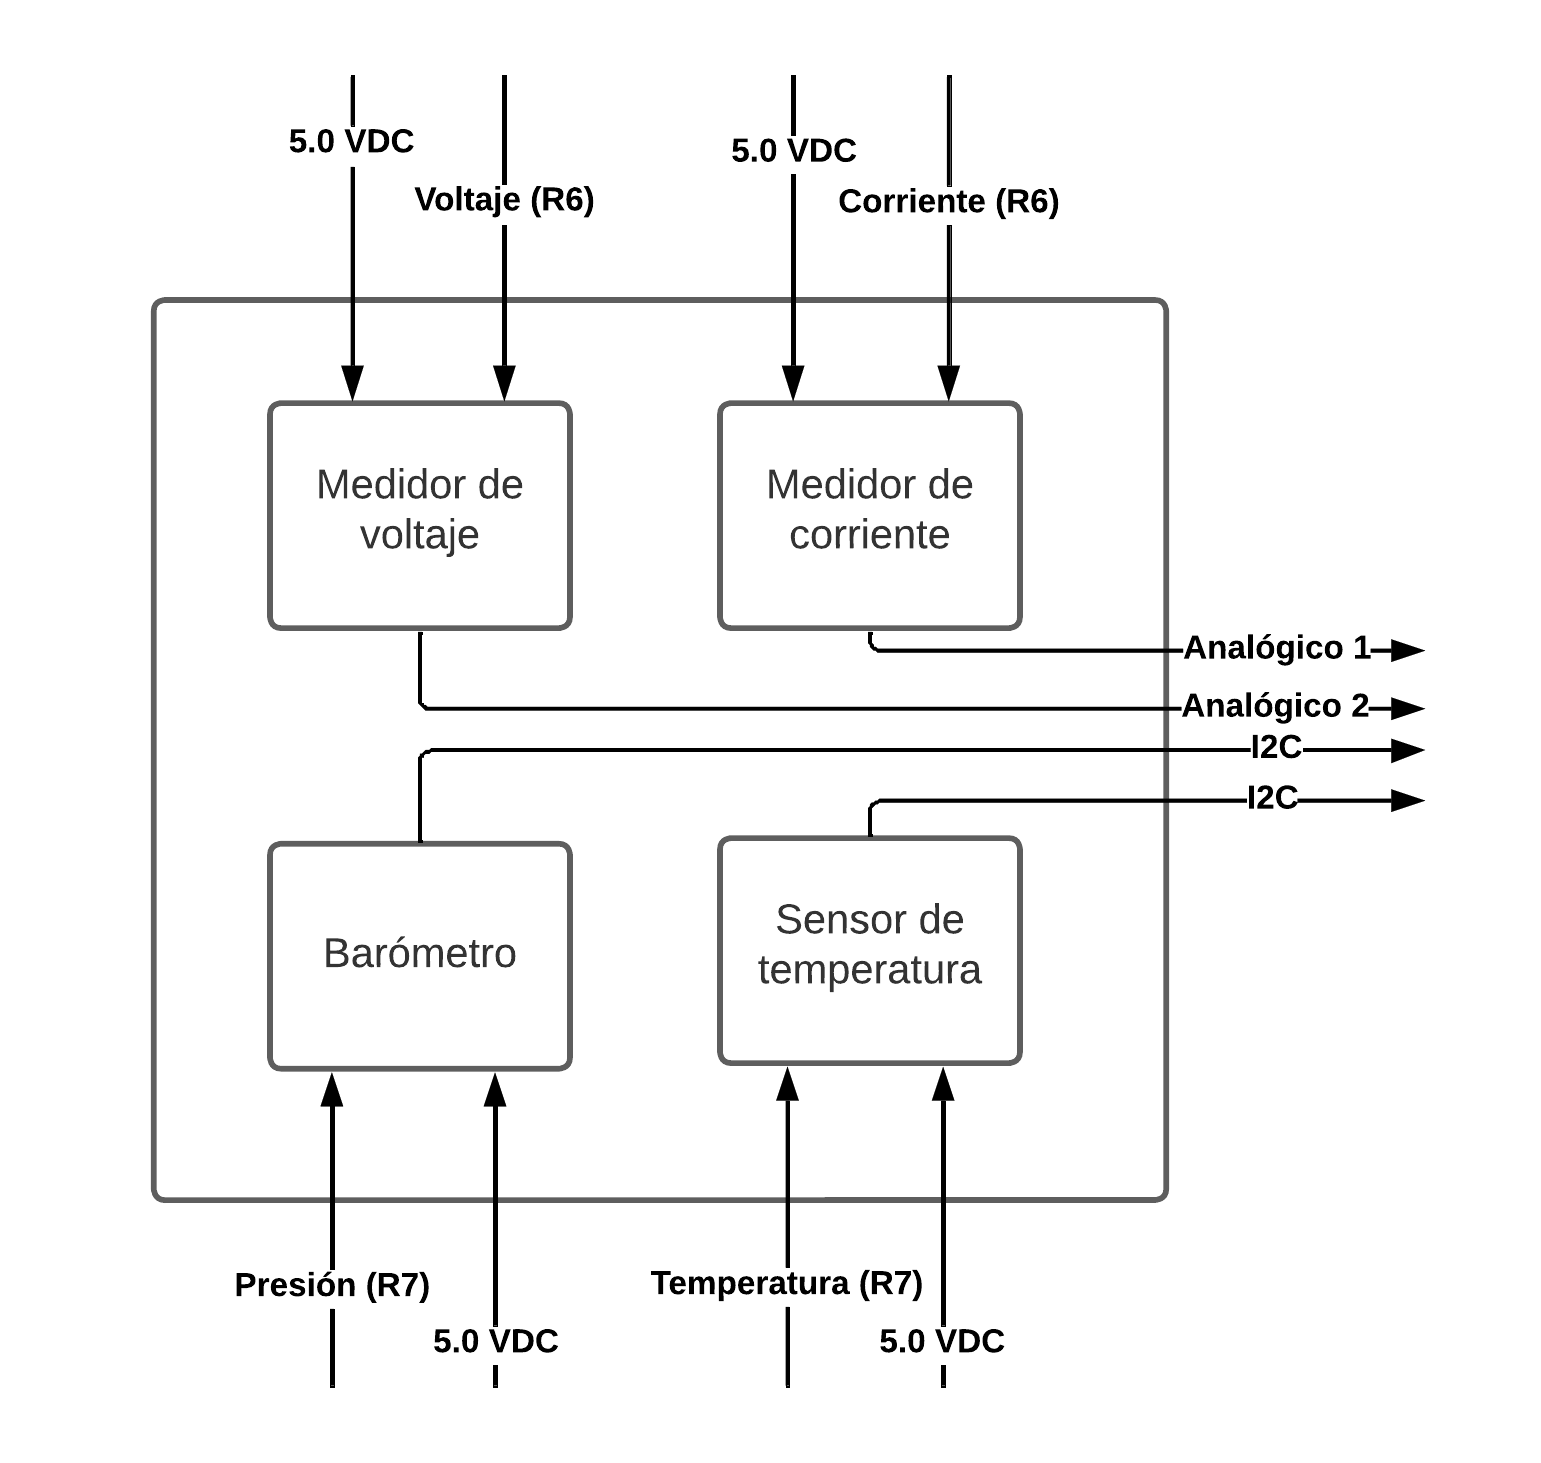
\includegraphics[width=0.6\textwidth]{Level2A.png} % Ajusta el tamaño según sea necesario
        \mycaption{Diagrama funcional nivel 2}
        \label{fig:level0DF}
    \end{figure}
\end{frame}



\newpage

\section{Diseño e Implementación}
%PAGINA 1

\begin{frame}
\frametitle{Diseño e Implementación}
\framesubtitle{Electrónica Digital}
Componentes de electrónica digital utilizados:
\begin{itemize}
    \item Microcontrolador: Arduino Nano.
    \item Datalogger: Openlog Sparkfun.
    \item Sensor barométrico y de temperatura: MS5611.
    \item Sensor de corriente por efecto Hall: ACS723.
\end{itemize}
\end{frame}



%PAGINA 4
\begin{frame}
    \frametitle{Diseño e Implementación}
    \framesubtitle{Etapa de potencia para carga útil}
    \vfill
    \begin{figure}
        \centering
        \begin{minipage}{.5\textwidth}
            \centering
            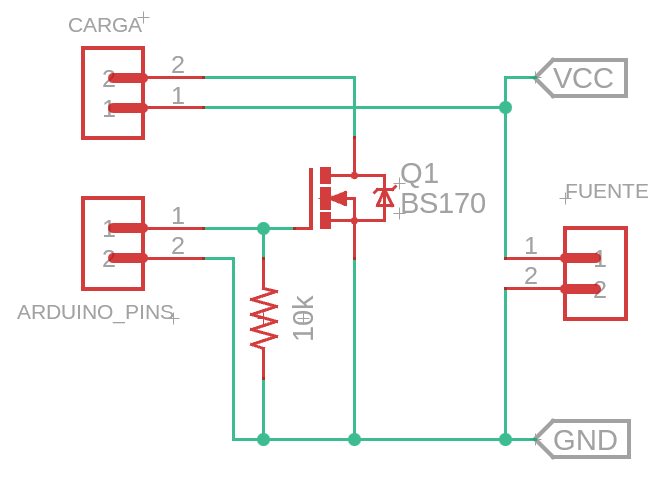
\includegraphics[width=0.6\textheight]{EtapaMosfet_Esquematico.png} % Reemplaza con tu primera imagen
            \mycaption{Esquemático de estapa con MOSFET BS170}
            \label{fig:ESQMOSFET}
        \end{minipage}\hfill
        \begin{minipage}{.5\textwidth}
            \centering
            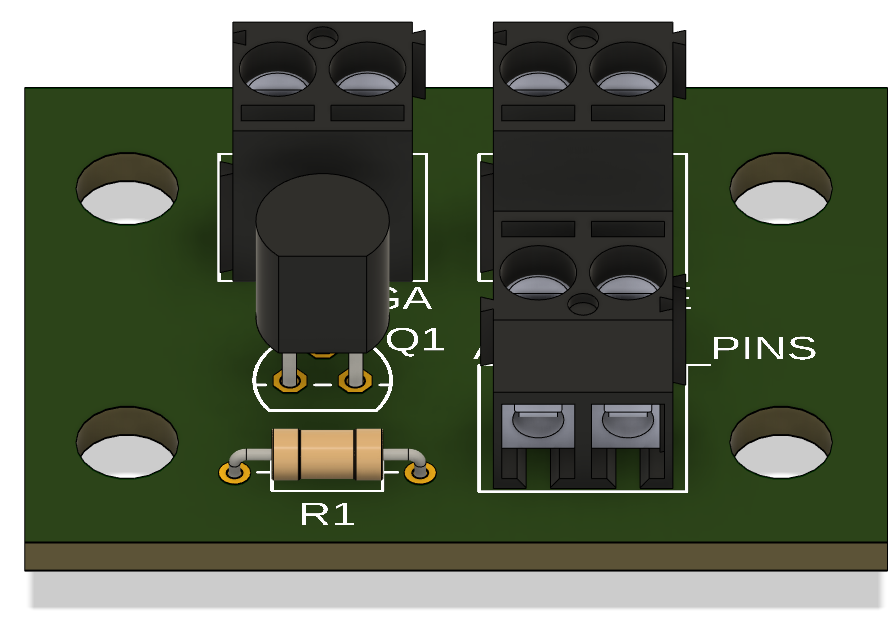
\includegraphics[width=.6\textheight]{3D_MOSFET.png} % Reemplaza con tu segunda imagen
            \mycaption{PCB de estapa con MOSFET BS170}
            \label{fig:PCBMOSFET}
        \end{minipage}
    \end{figure} 
\end{frame}


%PAGINA 6
\begin{frame}
    \frametitle{Diseño e Implementación}
    \framesubtitle{Baterías}
    \begin{figure}[H]
        \centering
        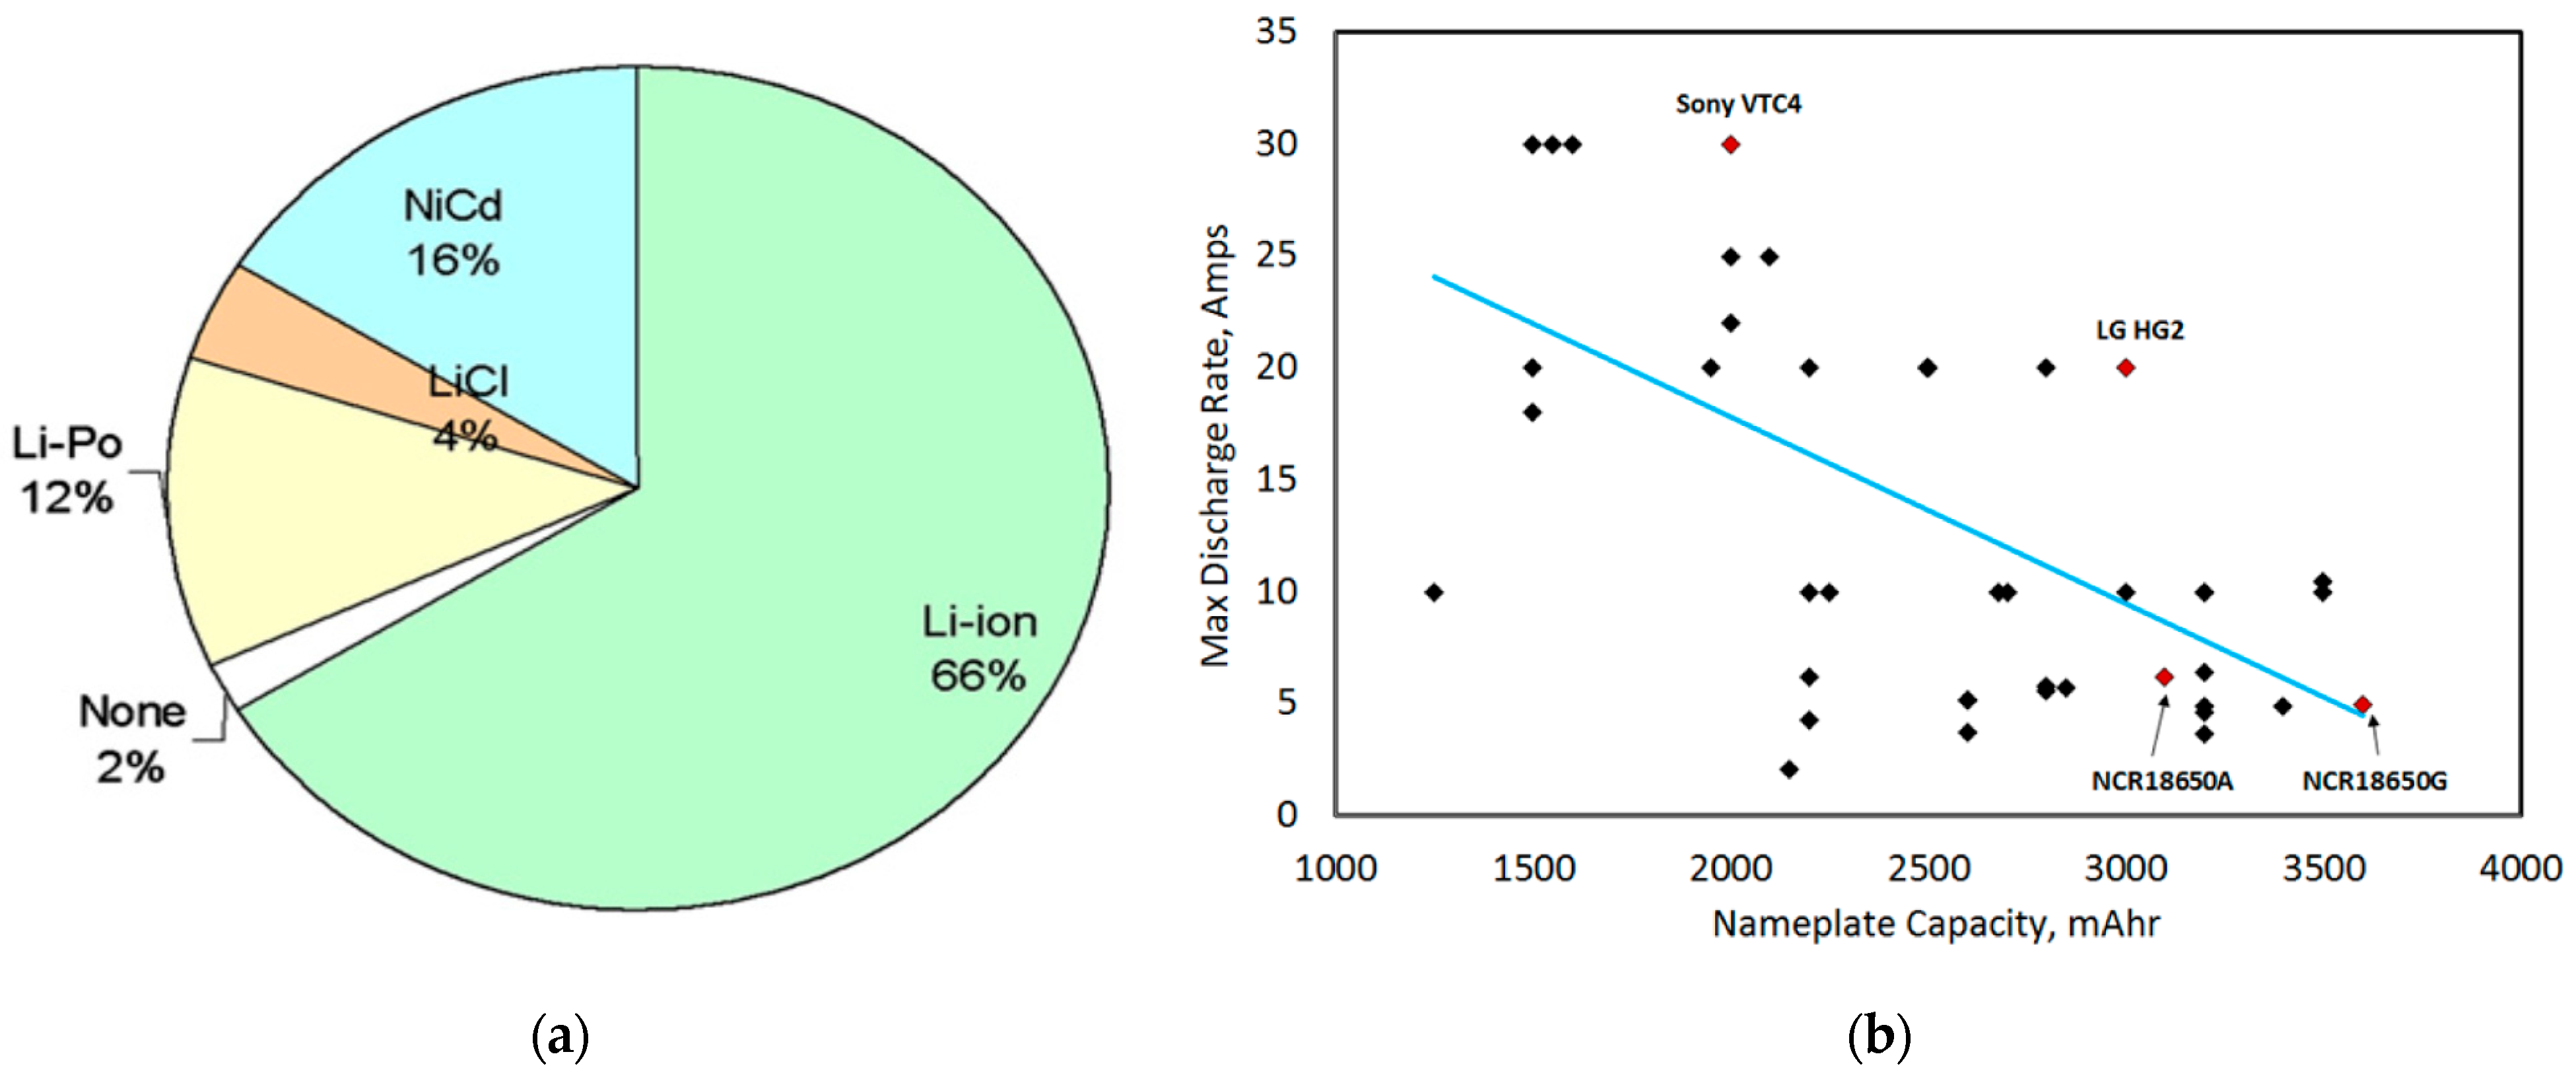
\includegraphics[width=0.8\textwidth]{COTSBatteries.png} % Ajusta el tamaño según sea necesario
        \mycaption{(a) Battery types used in pico- and nano-satellites[41]. (b) Summary of
        maximum discharge rate capabilities versus nameplate capacity of some representative
        COTS 18650 Li-ion cells \cite{chin2018energy}}
        \label{fig:COTSBatt}
    \end{figure}
    

\end{frame}


%PAGINA 7
\begin{frame}
    \frametitle{Diseño e Implementación}
    \framesubtitle{Baterías}
    Se seleccionó el modelo Panasonic NCR18650B por su corriente máxima de descarga de 4.9 A y capacidad nominal de 3400 mAh. Basándose en el presupuesto energético, se optó por un arreglo de 4 baterías. Para examinar la operatividad de etapas subsiguientes, como los convertidores DC-DC, se consideraron tres configuraciones: 
    \begin{itemize}
        \item 4s1p
        \item 2s2p
        \item 1s4p
    \end{itemize}
\end{frame}

%PAGINA 8
\begin{frame}
    \frametitle{Diseño e Implementación}
    \framesubtitle{Convertidores DC-DC}
    Aunque los convertidores lineales son baratos y simples, su eficiencia limitada, dada por $E = \frac{V_{\text{out}}}{V_{\text{in}}} \times 100\%$, conduce a una caída notable de eficiencia, como se ilustra en la Fig.\ref{fig:LDOE}.
    \begin{figure}[H]
        \centering
        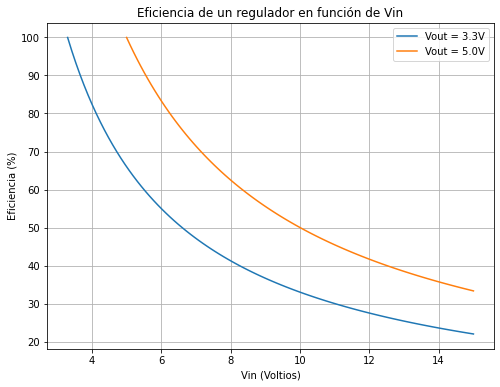
\includegraphics[width=0.5\textwidth]{Grafica_Eficiencia_LDO.png} % Ajusta el tamaño según sea necesario
        \mycaption{Eficiencia del regulador LT1117 en función del Vin}
        \label{fig:LDOE}
    \end{figure}
\end{frame}




%PAGINA 11

\begin{frame}
    \frametitle{Diseño e Implementación}
    \framesubtitle{Convertidores DC-DC: Arreglo 4s1p}
    \begin{figure}[H]
        \centering
        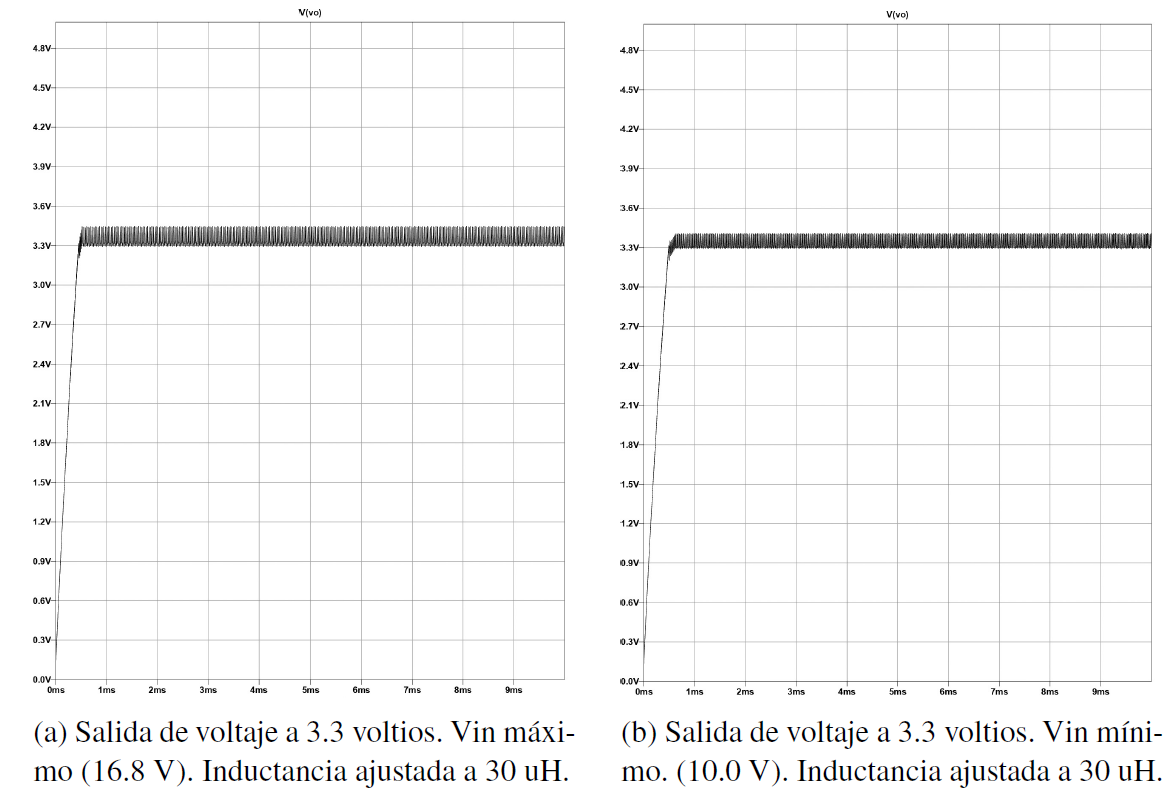
\includegraphics[width=0.7\textwidth]{4S1P_A.png} % Ajusta el tamaño según sea necesario
        \mycaption{Convertidor DC-DC MC34063A, arreglo 4s1p, bus de 3.3 V a 750 mA.}
        \label{fig:4S1P_A}
    \end{figure}
\end{frame}

%PAGINA 16

\begin{figure}
    \frametitle{Diseño e Implementación}
    \framesubtitle{Convertidores DC-DC: Esquemático Bus 3.3 V}
    \begin{figure}[H]
        \centering
        \includegraphics[width=0.9\textwidth]{MC34063A_Esquemático_33V.png} % Ajusta el tamaño según sea necesario
        \mycaption{Convertidor DC-DC MC34063A, arreglo 4s1p, bus de 3.3 V a 750 mA.}
        \label{fig:Resultado3.3}
    \end{figure}
\end{figure}


%PAGINA 12
\begin{frame}
    \frametitle{Diseño e Implementación}
    \framesubtitle{Convertidores DC-DC: Arreglo 4s1p}
    \begin{figure}[H]
        \centering
        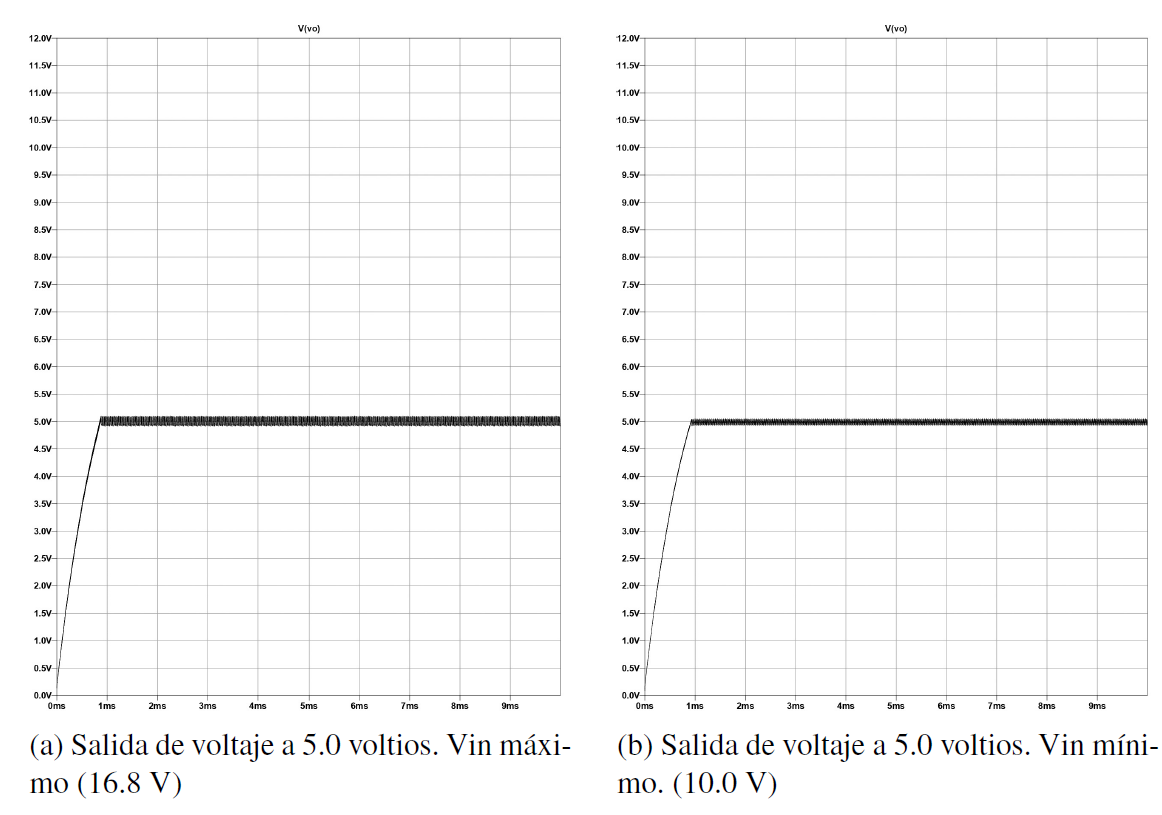
\includegraphics[width=0.7\textwidth]{4S1P_B.png} % Ajusta el tamaño según sea necesario
        \mycaption{Convertidor DC-DC MC34063A, arreglo 4s1p, bus de 5.0 V a 750 mA.}
        \label{fig:4S1P_B}
    \end{figure}
\end{frame}




%PAGINA 17

\begin{figure}
    \frametitle{Diseño e Implementación}
    \framesubtitle{Convertidores DC-DC: Esquemático Bus 5.0 V}
    \begin{figure}[H]
        \centering
        \includegraphics[width=0.9\textwidth]{MC34063A_Esquemático_50V.png} % Ajusta el tamaño según sea necesario
        \mycaption{Convertidor DC-DC MC34063A, arreglo 4s1p, bus de 5.0 V a 750 mA.}
        \label{fig:Resultado5.0}
    \end{figure}
\end{figure}


%PAGINA 17
\begin{frame}
\frametitle{Diseño e Implementación}
\framesubtitle{Circuito de Protección: Limitador de corriente}
\begin{figure}
    \begin{figure}[b]
        \centering
        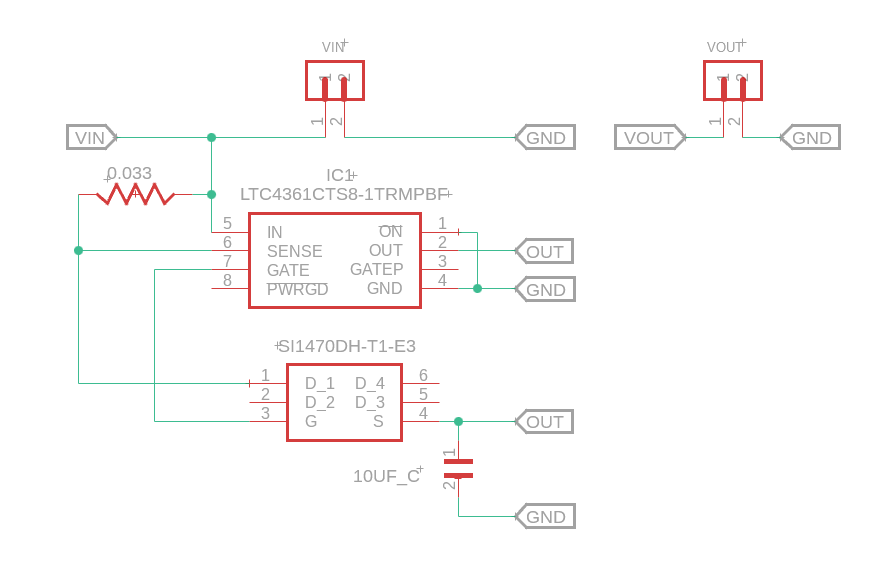
\includegraphics[width=0.75\textwidth]{Esquematico_LTC4361.png} % Ajusta el tamaño según sea necesario     
        \mycaption{Circuito de protección LTC4361. \( R_{\text{sense}} = 0.033\,\Omega \) para \( I_{\text{trip}} = 1.5\,A \). PCB de material FR-4 (0.762\,mm), \( I_{\text{máx}} = 2\,A \) \cite{LTC4361}\cite{altiumfr4}.}
        \label{fig:Resultado6.0}
    \end{figure}
\end{figure}
\end{frame}
\newpage

\section{Integración}
%PAGINA 6

\begin{frame}
    \frametitle{Integración del Sistema: Hardware}
    \begin{figure}[H]
        \centering
        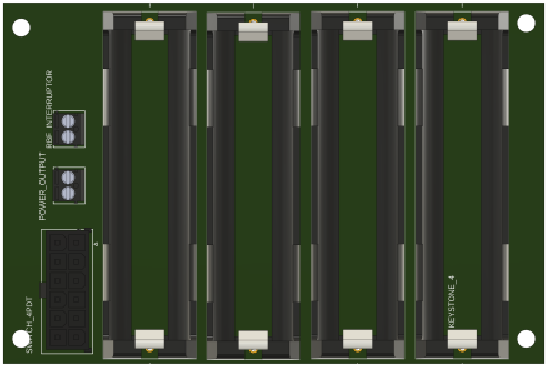
\includegraphics[width=0.8\textwidth]{EPS_FINAL4.png} % Ajusta el tamaño según sea necesario
        \mycaption{PCB 1 del EPS}
        \label{fig:PCB1Final}
    \end{figure}
\end{frame}

%PAGINA 7

\begin{frame}
    \frametitle{Integración del Sistema: Hardware}

    \begin{figure}[H]
        \centering
        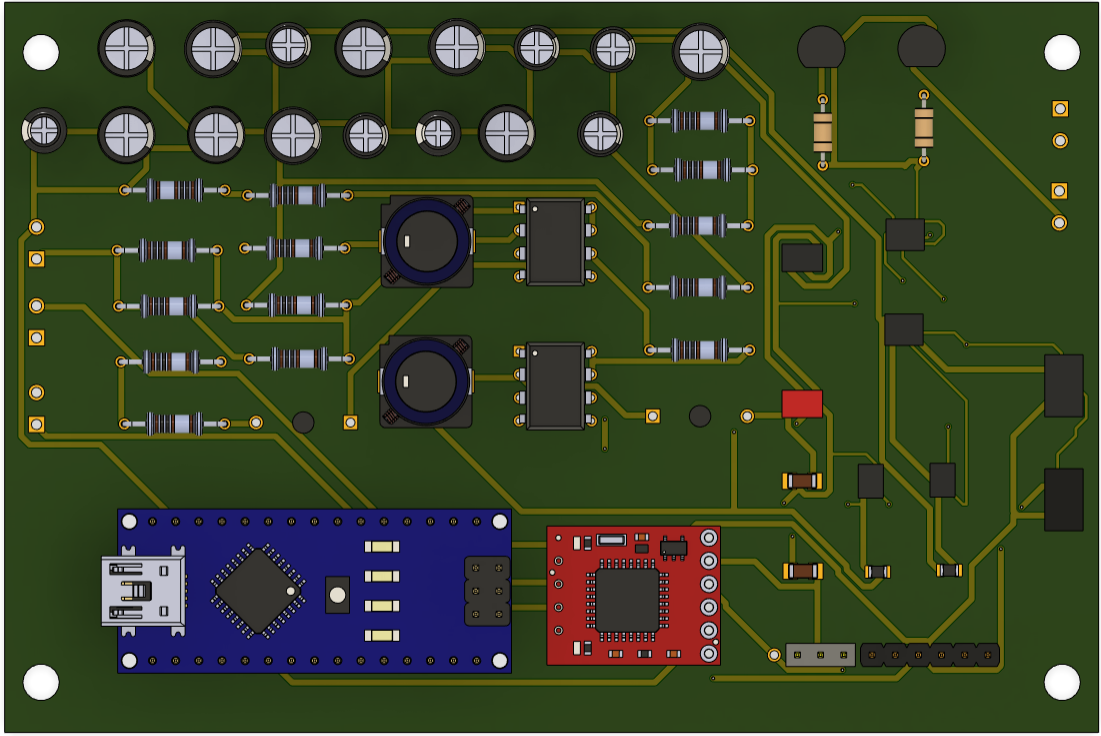
\includegraphics[width=0.8\textwidth]{EPS_FINAL.png}
        \mycaption{PCB 2 del EPS}
        \label{fig:PCB2Final}
    \end{figure}
\end{frame}


%PAGINA FINAL

\begin{frame}
    \frametitle{Integración del Sistema: Software}

    \begin{figure}[H]
        \centering
        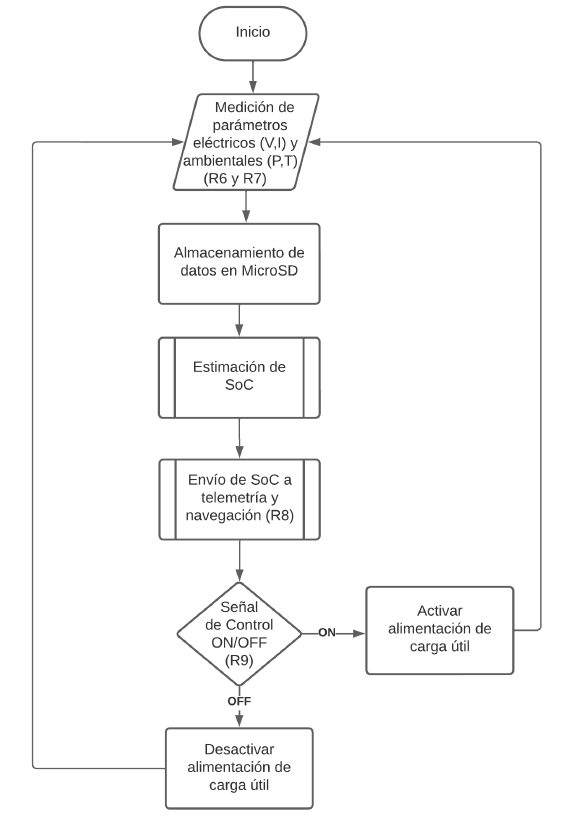
\includegraphics[width=0.4\textwidth]{Flujograma.png} % Ajusta el tamaño según sea necesario
        \mycaption{Flujograma de algoritmo de EPS.}
        \label{fig:Flujograma}
    \end{figure}
\end{frame}

\newpage

\section{Verificación}
%PAGINA 1

\begin{frame}
    \frametitle{Validación del Sistema}
    \begin{figure}[H]
        \centering
        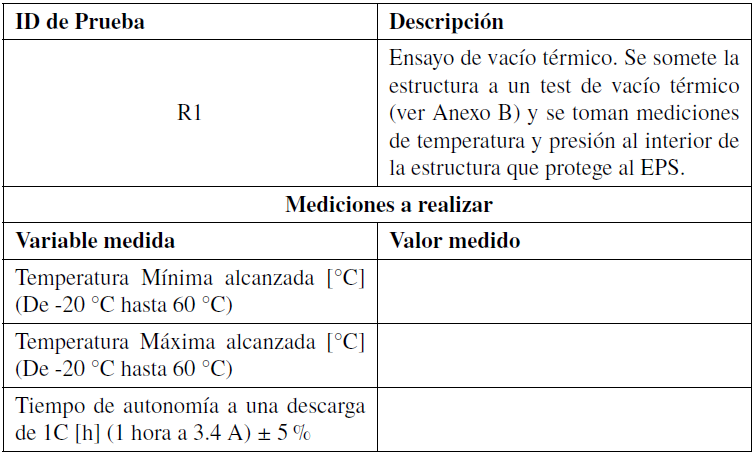
\includegraphics[width=\textwidth]{V1.png} % Ajusta el tamaño según sea necesario
        \mycaption{Prueba ambiental.}
        \label{fig:V1}
    \end{figure}
\end{frame}


%PAGINA 2

\begin{frame}
    \frametitle{Validación del Sistema}
    \begin{figure}[H]
        \centering
        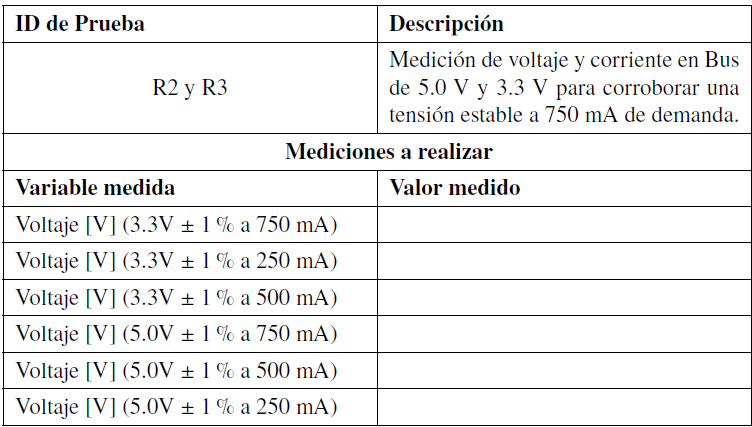
\includegraphics[width=\textwidth]{V2.png} % Ajusta el tamaño según sea necesario
        \mycaption{Prueba de parámetros eléctricos del EPS.}
        \label{fig:V2}
    \end{figure}
\end{frame}

%PAGINA 3

\begin{frame}
    \frametitle{Validación del Sistema}
    \begin{figure}[H]
        \centering
        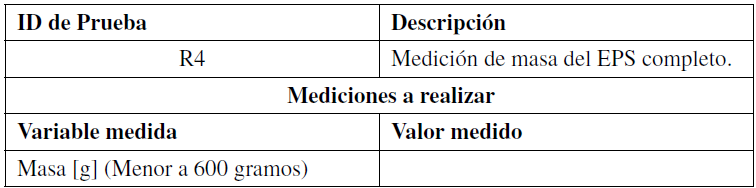
\includegraphics[width=\textwidth]{V3.png} % Ajusta el tamaño según sea necesario
        \mycaption{Prueba de masa}
        \label{fig:V3}
    \end{figure}
\end{frame}

%PAGINA 4

\begin{frame}
    \frametitle{Validación del Sistema}
    \begin{figure}[H]
        \centering
        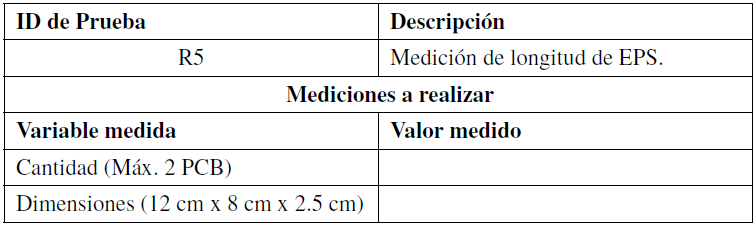
\includegraphics[width=\textwidth]{V4.png} % Ajusta el tamaño según sea necesario
        \mycaption{Prueba de longitud de PCBs.}
        \label{fig:V4}
    \end{figure}
\end{frame}

%PAGINA 5

\begin{frame}
    \frametitle{Validación del Sistema}
    \begin{figure}[H]
        \centering
        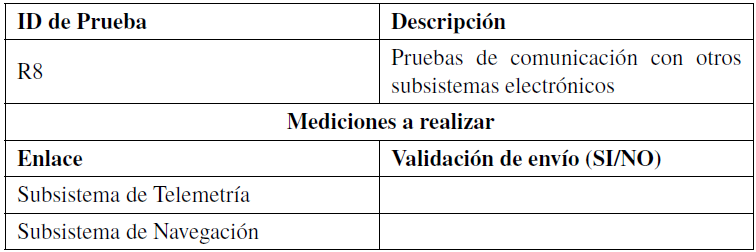
\includegraphics[width=\textwidth]{V5.png} % Ajusta el tamaño según sea necesario
        \mycaption{Pruebas de comunicación.}
        \label{fig:V5}
    \end{figure}
\end{frame}


%PAGINA 6

\begin{frame}
    \frametitle{Validación del Sistema}
    \begin{figure}[H]
        \centering
        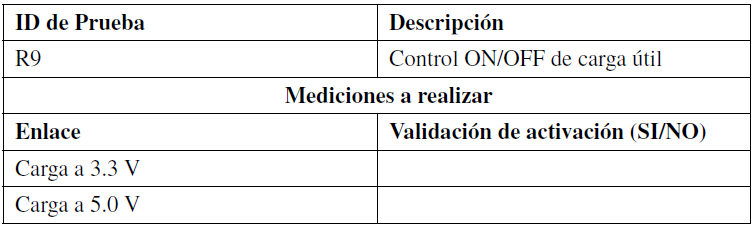
\includegraphics[width=\textwidth]{V6.png} % Ajusta el tamaño según sea necesario
        \mycaption{Prueba de control ON/OFF de carga útil}
        \label{fig:V6}
    \end{figure}
\end{frame}

%PAGINA 7

\begin{frame}
    \frametitle{Validación del Sistema}
    \begin{figure}[H]
        \centering
        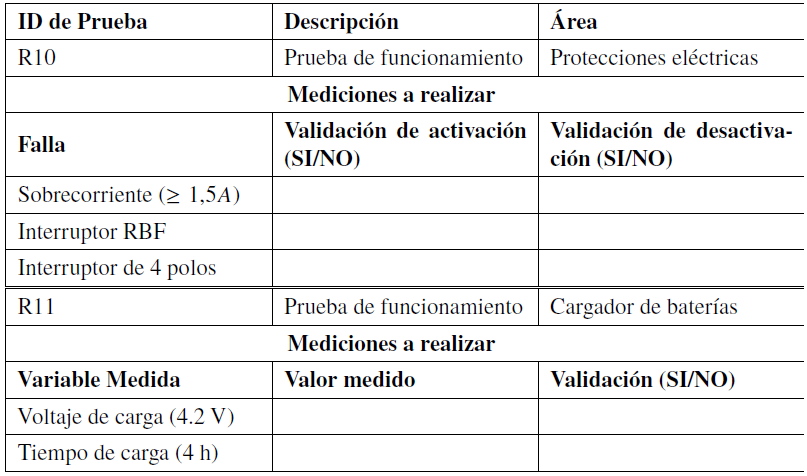
\includegraphics[width=0.90\textwidth]{V7.png} % Ajusta el tamaño según sea necesario
        \mycaption{Pruebas de protecciones eléctricas y cargador.}
        \label{fig:V7}
    \end{figure}
\end{frame}

\newpage

\section{Conclusiones}
%PAGINA 1

\begin{frame}
\frametitle{Conclusiones}
En resumen, esta investigación ha aportado al campo de sistemas de energía para sondas de HAB, aplicando la metodología de proyectos de la NASA.\\
\vspace{0.5 cm}
Al cumplir con los objetivos específicos, hemos avanzado en la comprensión de las condiciones ambientales para la misión, establecido requisitos eléctricos precisos, diseñado una arquitectura lógica y física para el sistema de energía, y desarrollado un plan de pruebas.\\
\vspace{0.5 cm}
Este enfoque de investigación, centrado en el uso de tecnología comercial, software libre y complejidad controlada, abre nuevas perspectivas en la exploración de la región Near-Space.
\end{frame}

\newpage


%--------- CUERPO DE LA PRESENTACION --------





%--------- PREGUNTAS Y RESPUESTAS -----------
\section{Q\&A}
\begin{frame}
\begin{tikzpicture}[remember picture, overlay]
    \node[opacity=0.19, anchor=south] at (current page.south) {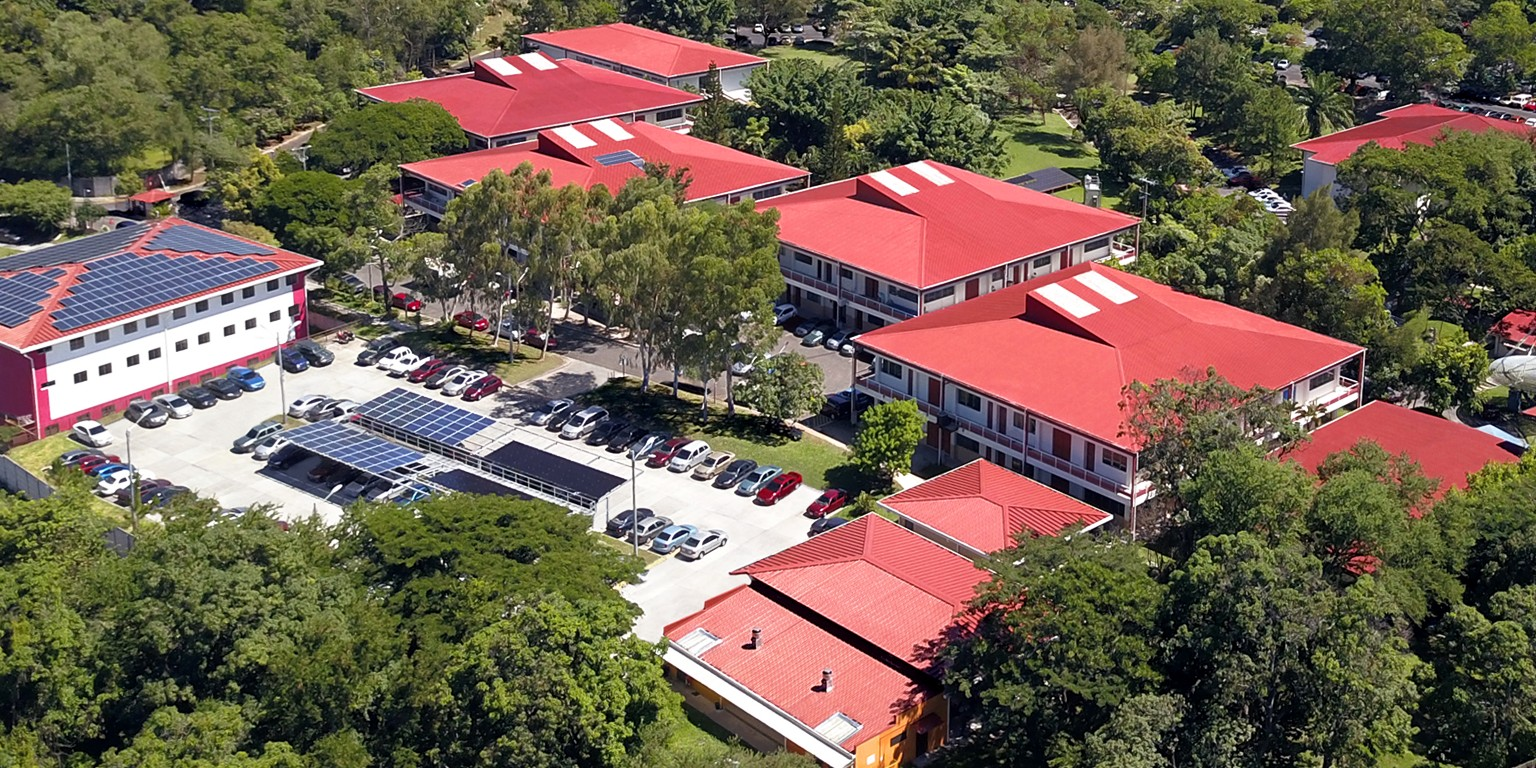
\includegraphics[width=\paperwidth,height=0.89\paperheight]{images/CampusUDB.jpg}};
\end{tikzpicture}

\begin{center}
\Huge{\textbf{Preguntas y Respuestas}}
\end{center}
\vfill

\end{frame}

\newpage

\appendix
\section*{Anexos}

% Página 1
\begin{frame}
    \frametitle{Anexo 1}
    \framesubtitle{Limitaciones: EPS}
    \begin{itemize}
        \small
        \item Recursos financieros: Se recurrió a software libre debido al alto costo de las licencias de software de pago.
        \item Tiempo: El proyecto estaba programado para desarrollarse en un periodo limitado de aproximadamente 16 semanas.
        \item Pruebas en laboratorio: La ausencia de equipo especializado, en particular una cámara de vacío térmico, limitó la realización de pruebas experimentales.
        \item Simulaciones: El uso del modelo GFS y el estándar atmosférico ISA, aunque valiosos, tienen limitaciones que pueden afectar la precisión de los resultados.
    \end{itemize}
\end{frame}


% Página 2
\begin{frame}
    \frametitle{Anexo 2}
    \framesubtitle{Antecedentes: EPS}
    \begin{figure}
        \centering
        \begin{minipage}{.5\textwidth}
            \centering
            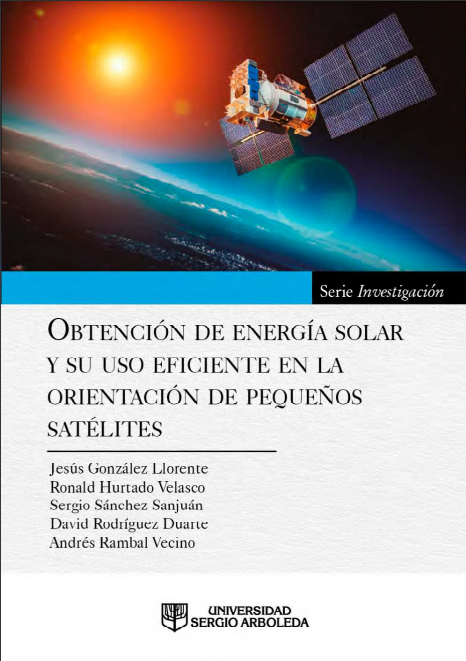
\includegraphics[width=0.38\textheight]{LibroEnergiaSatelites.png} % Reemplaza con tu primera imagen
            \mycaption{Libro ''Obtención de Energía Solar y su Uso Eficiente en la Orientación de Pequeños Satélites'' \cite{energiasat1}}
            \label{fig:sat1}
        \end{minipage}\hfill
        \begin{minipage}{.5\textwidth}
            \centering
            
\includegraphics[width=0.65\textheight]{Birds_logo.png} % Reemplaza con tu segunda imagen
            \vspace*{0.25 cm}
            \mycaption{Proyecto Birds del Kyushu Institute of Technology \cite{jara2022orbit}}
            \label{fig:sat2}
        \end{minipage}
    \end{figure}
    \end{frame}

% Página 3

\begin{frame}
    \frametitle{Anexo 2}
    \framesubtitle{Antecedentes: EPS}
    \begin{figure}
        \centering
        \begin{minipage}{.5\textwidth}
            \centering
            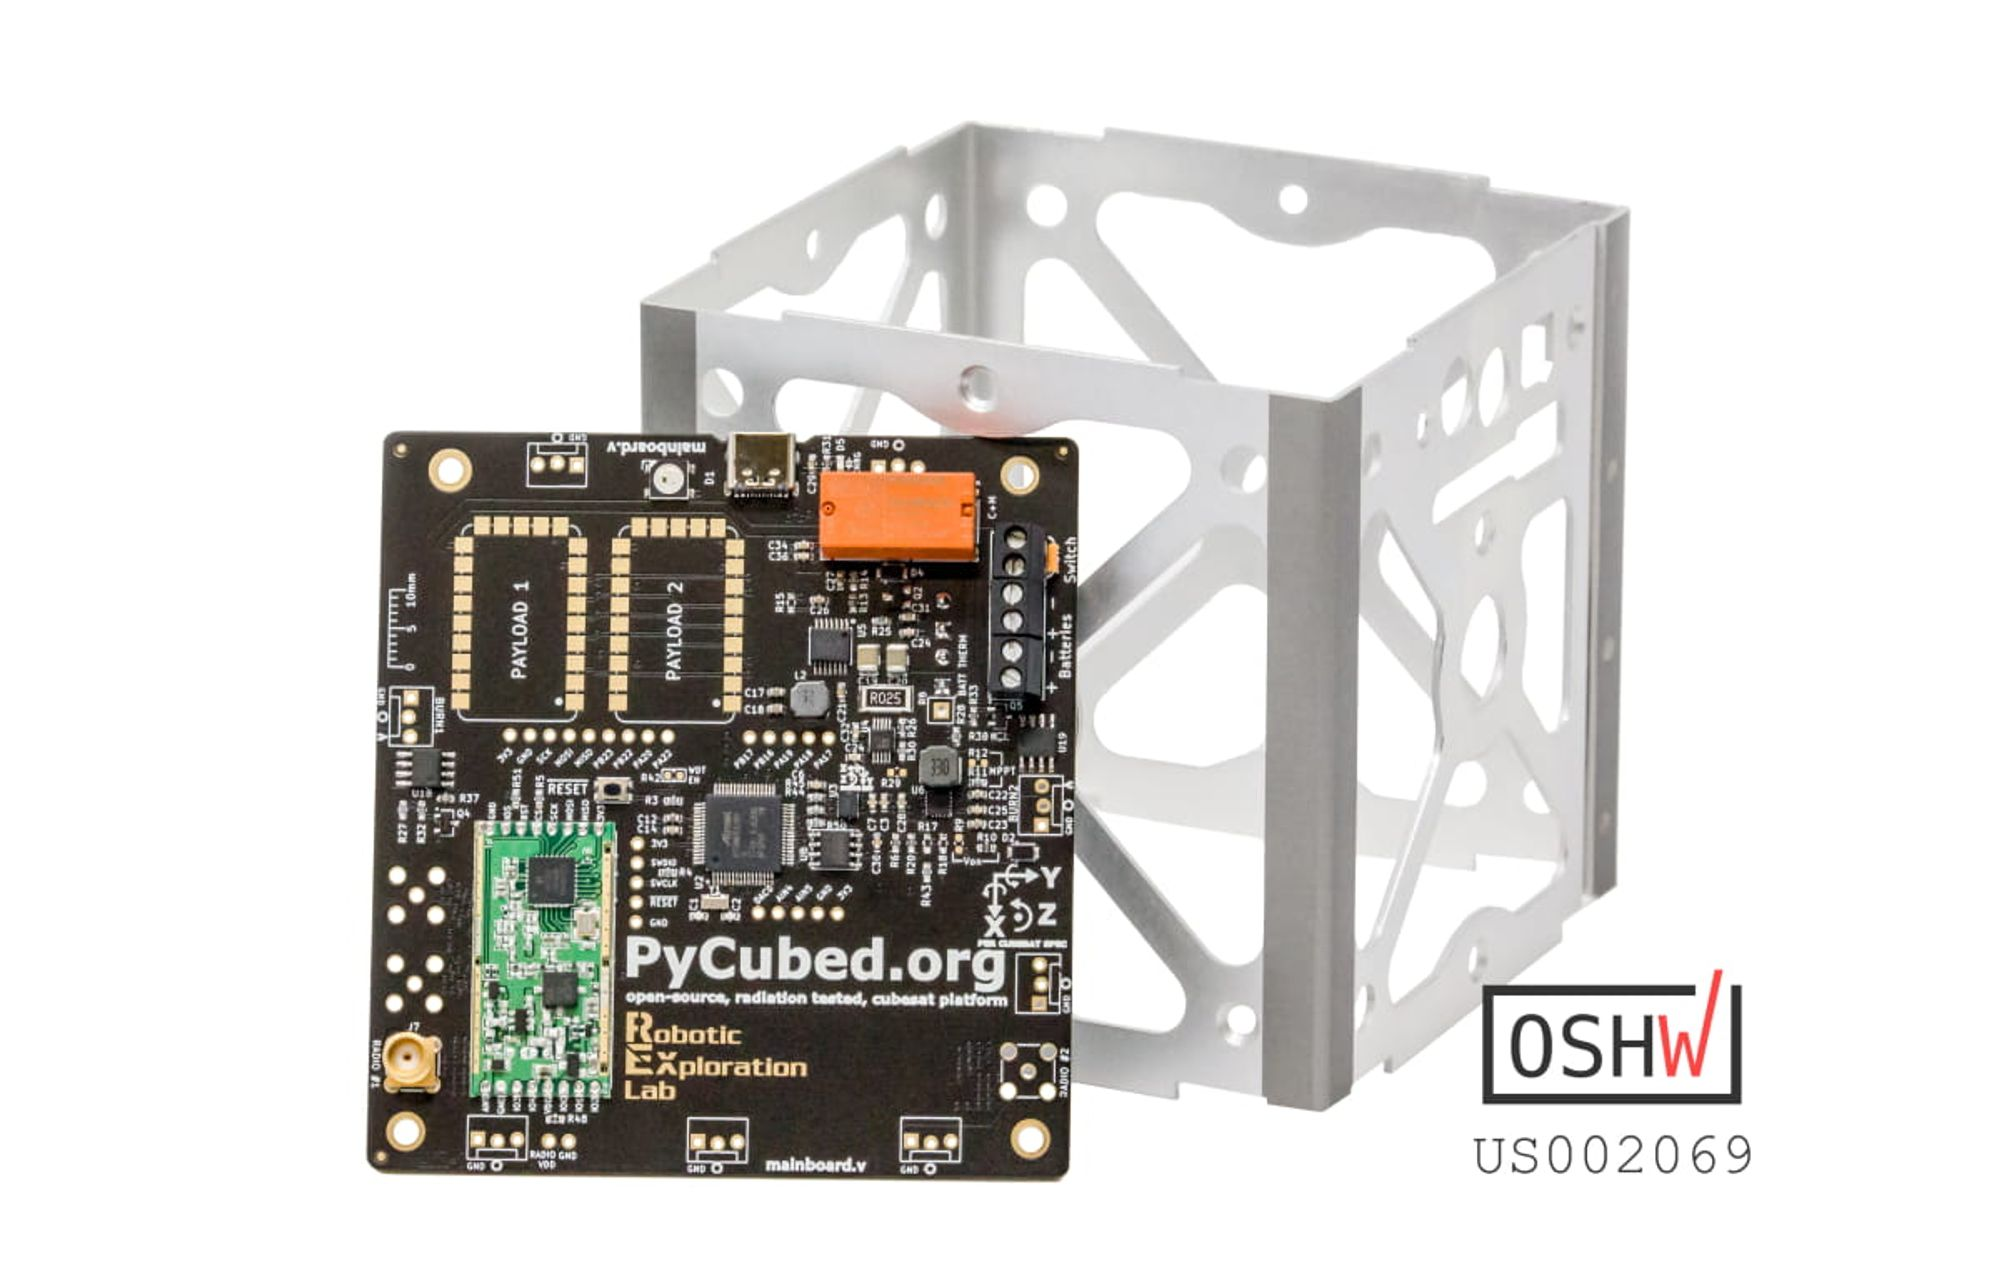
\includegraphics[width=0.75\textheight]{pycubed.jpg} % Reemplaza con tu primera imagen
            \mycaption{Proyecto Pycubed de la Universidad de Stanford \cite{pycubed}}
            \label{fig:sat3}
        \end{minipage}\hfill
        \begin{minipage}{.5\textwidth}
            \centering
            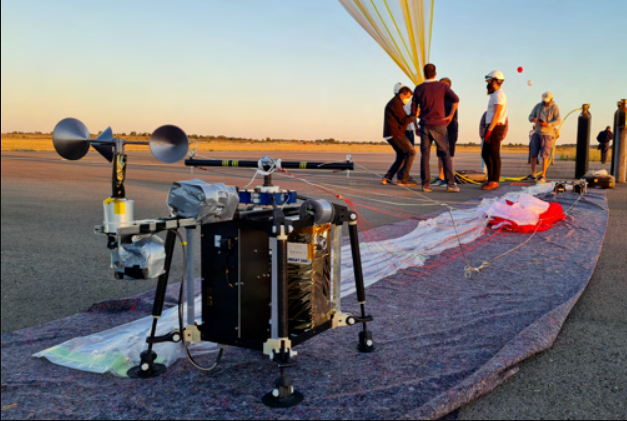
\includegraphics[width=.6\textheight]{TASEC_Lab.png} % Reemplaza con tu segunda imagen
            \vspace*{0.5 cm}
            \mycaption{Proyecto TASEC-Lab de la Universidad Politécnica de Madrid \cite{TASEC}}
            \label{fig:sat4}
        \end{minipage}
    \end{figure}    
    \end{frame}


% Página 4

\begin{frame}
    \frametitle{Anexo 3}
    \framesubtitle{Diseño: Relé, BJT, MOSFET}
    Se seleccionó un MOSFET, específicamente el modelo BS170, para el circuito de potencia, descartando relés debido a su alta disipación energética. Los MOSFET, siendo dispositivos de coeficiente térmico positivo (PTC) y controlados por voltaje, ofrecen una eficiencia superior a los BJT.
    \begin{figure}[H]
        \centering
        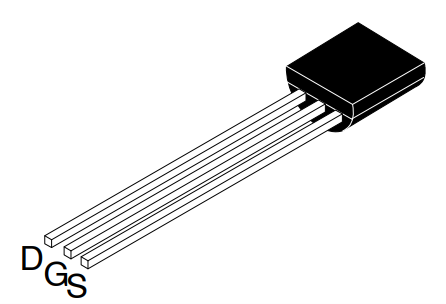
\includegraphics[width=0.4\textwidth]{BS170_Pinout.png} % Ajusta el tamaño según sea necesario
        \mycaption{MOSFET modelo BS170}
        \label{fig:BS170MOSFET}
    \end{figure}
    
    \end{frame}
    
    %PAGINA 5
    
    \begin{frame}
        \frametitle{Anexo 3}
        \framesubtitle{Diseño: Relé, BJT, MOSFET}
        \begin{figure}
            \centering
            \begin{minipage}{.5\textwidth}
                \centering
                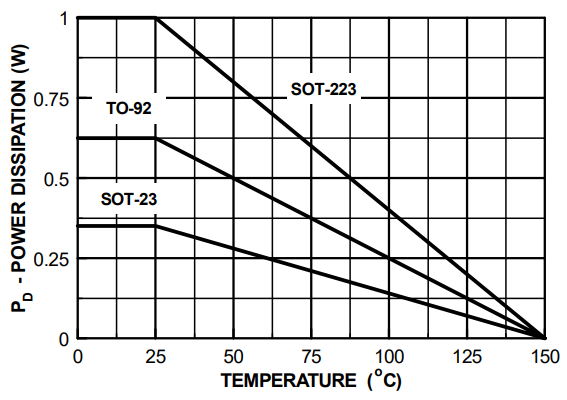
\includegraphics[width=0.65\textheight]{2N2222ApowerD.png} % Reemplaza con tu primera imagen
                \mycaption{Variación de potencia disipada en el 2N2222A en función de la
                temperatura ambiente}
                \label{fig:RESBJT}
            \end{minipage}\hfill
            \begin{minipage}{.5\textwidth}
                \centering
                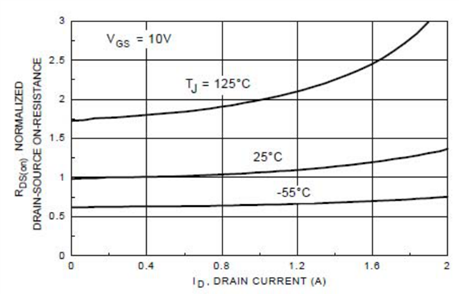
\includegraphics[width=.70\textheight]{resvscorriente.png} % Reemplaza con tu segunda imagen
                \mycaption{Variación de la resistencia interna en función de la corriente a distintas
                temperaturas ambiente.}
                \label{fig:RESMOSFET}
            \end{minipage}
        \end{figure}  
    \end{frame}
    

% Página 6 

\begin{frame}
    \frametitle{Anexo 4}
    \framesubtitle{Diseño: Simulación 4s1p, bus 3.3V}
    \begin{figure}[H]
        \centering
        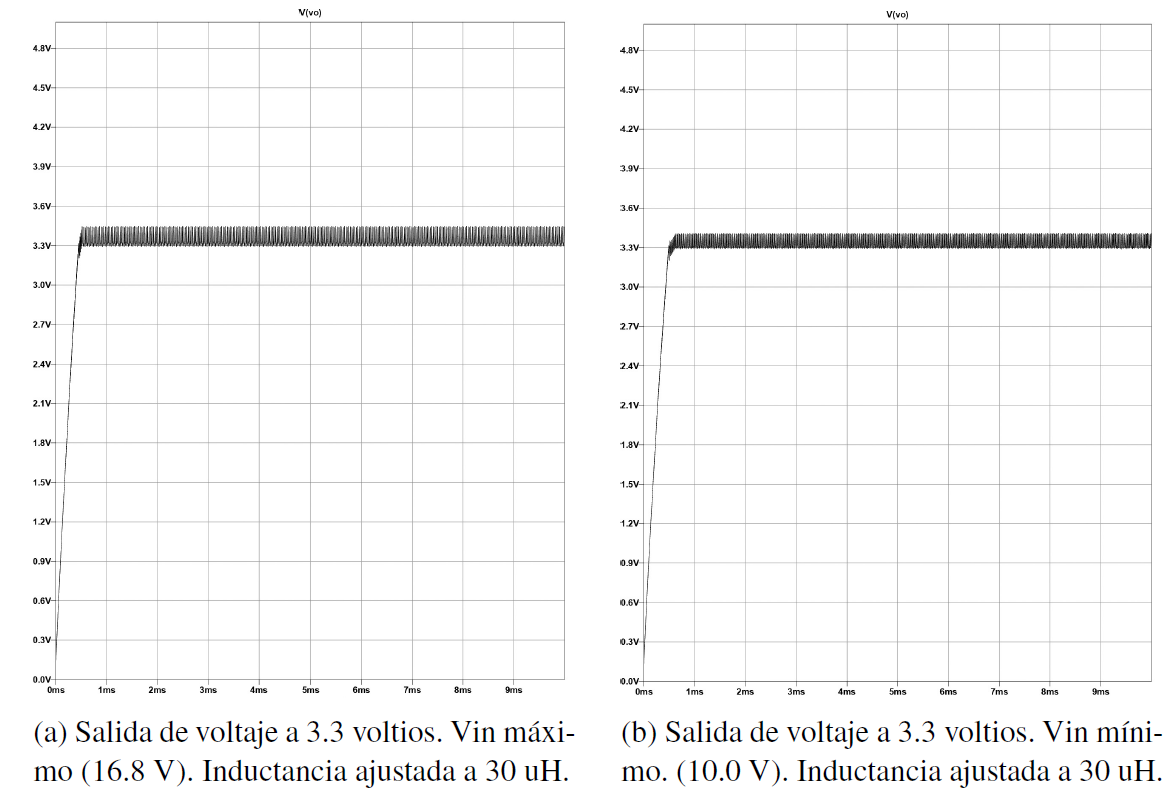
\includegraphics[width=0.7\textwidth]{4S1P_A.png} % Ajusta el tamaño según sea necesario
        \mycaption{Convertidor DC-DC MC34063A, arreglo 4s1p, bus de 3.3 V a 750 mA.}
        \label{fig:4S1P_A}
    \end{figure}
\end{frame}

%PAGINA 7
\begin{frame}
    \frametitle{Anexo 4}
    \framesubtitle{Diseño: Simulación 4s1p, bus 5.0V}
    \begin{figure}[H]
        \centering
        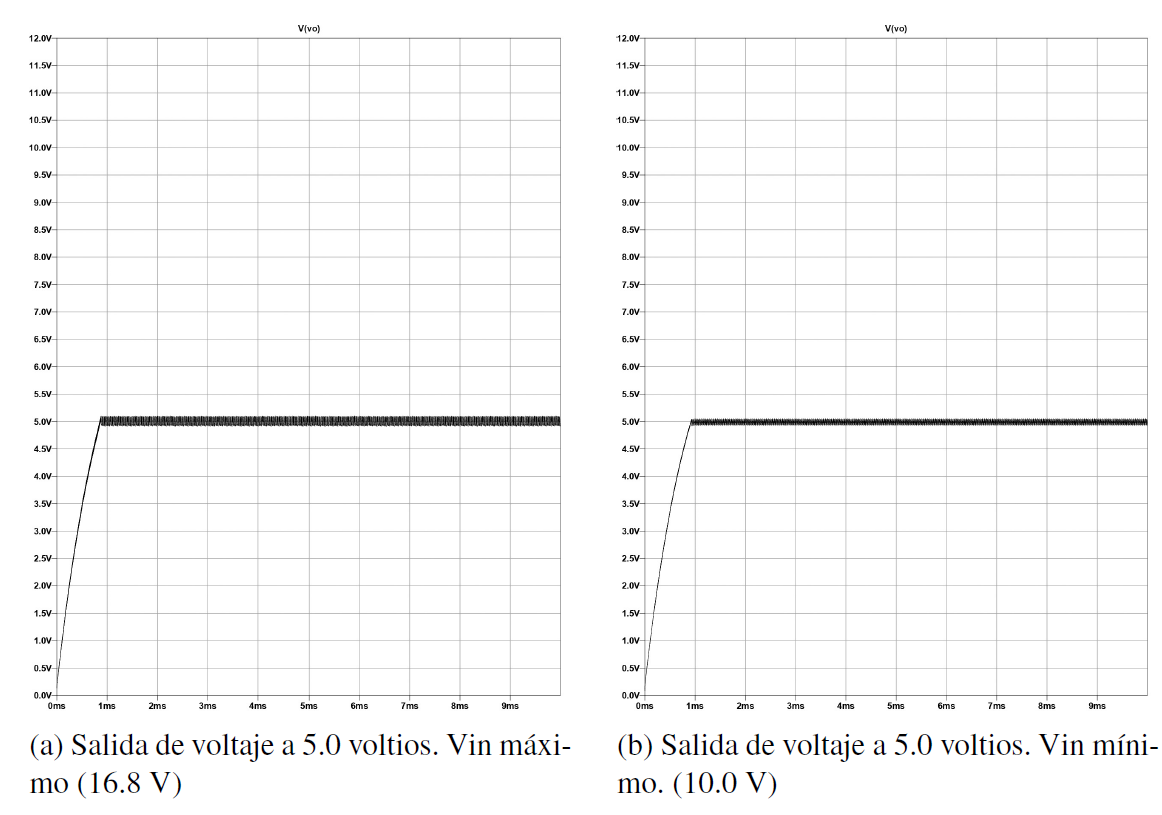
\includegraphics[width=0.7\textwidth]{4S1P_B.png} % Ajusta el tamaño según sea necesario
        \mycaption{Convertidor DC-DC MC34063A, arreglo 4s1p, bus de 5.0 V a 750 mA.}
        \label{fig:4S1P_B}
    \end{figure}
\end{frame}

%PAGINA 8
\begin{frame}
    \frametitle{Anexo 4}
    \framesubtitle{Diseño: Simulación 2s2p, bus 3.3V}
    \begin{figure}[H]
        \centering
        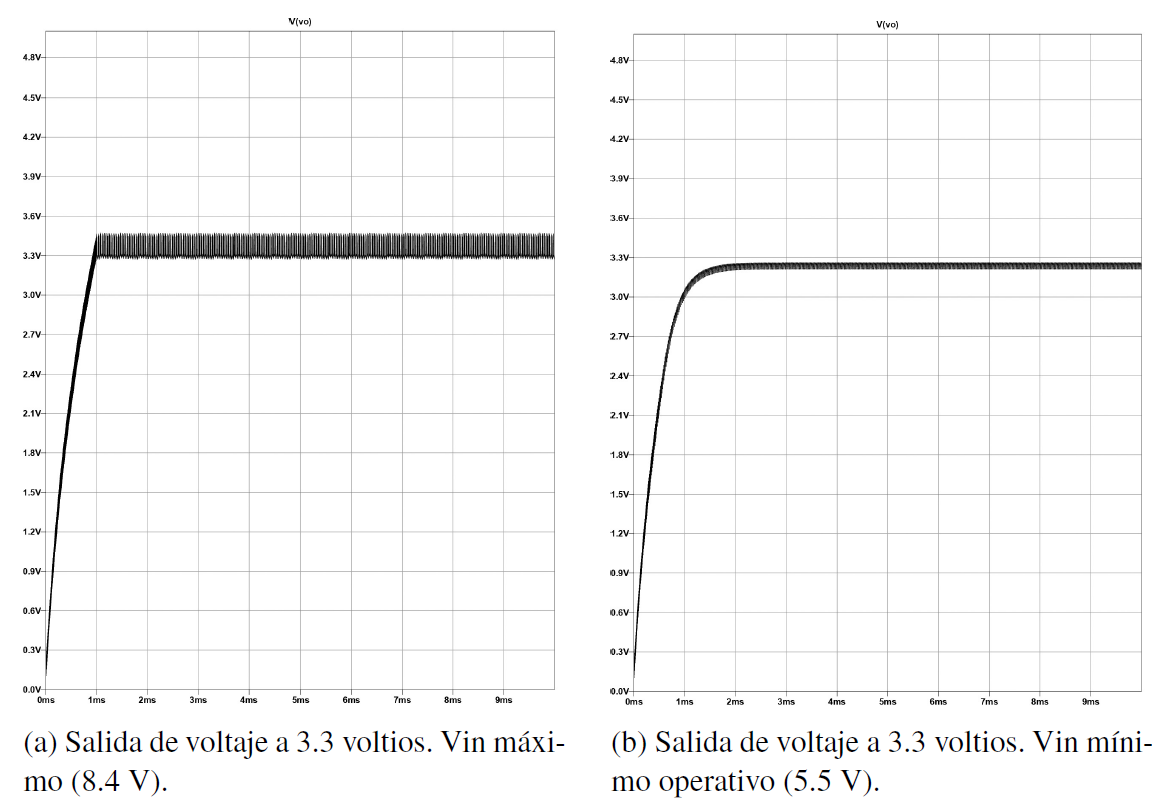
\includegraphics[width=0.7\textwidth]{2S2P_A.png} % Ajusta el tamaño según sea necesario
        \mycaption{Convertidor DC-DC MC34063A, arreglo 2s2p, bus de 3.3 V a 750 mA.}
        \label{fig:2S2P_A}
    \end{figure}
\end{frame}

%PAGINA 9
\begin{frame}
    \frametitle{Anexo 4}
    \framesubtitle{Diseño: Simulación 2s2p, bus 5.0V}
    \begin{figure}[H]
        \centering
        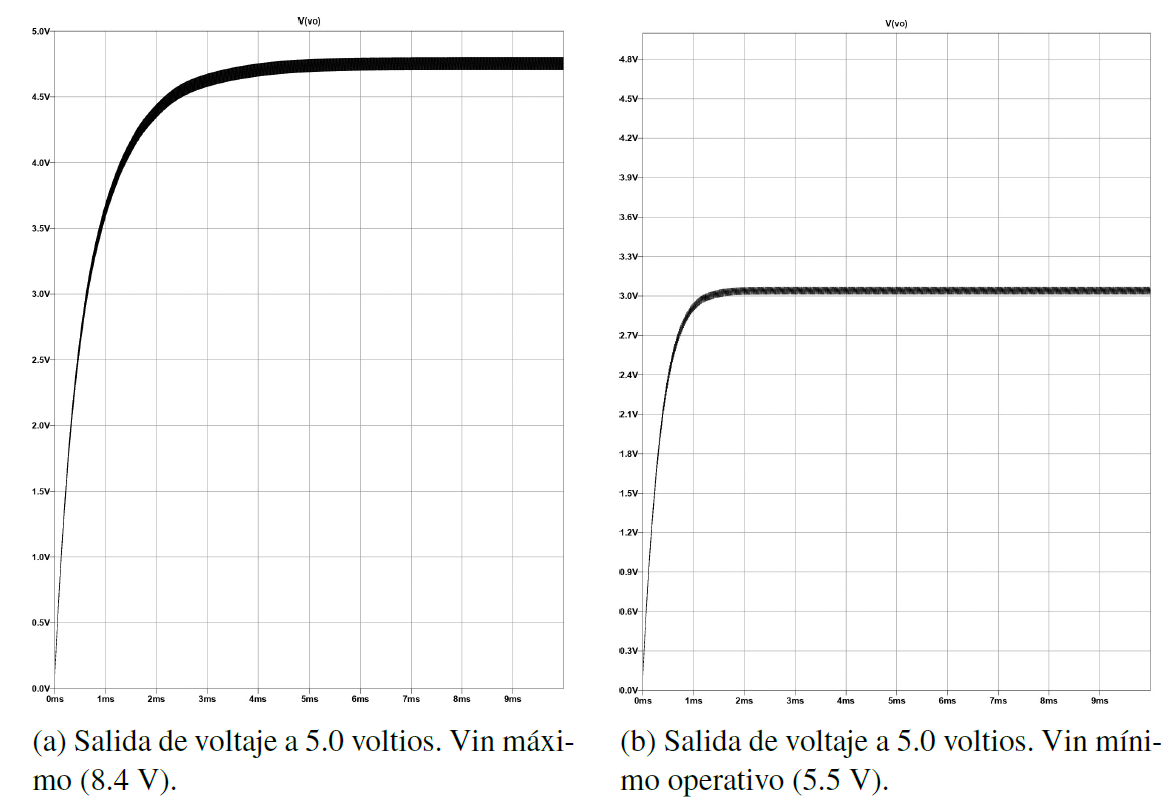
\includegraphics[width=0.7\textwidth]{2S2P_B.png} % Ajusta el tamaño según sea necesario
        \mycaption{Convertidor DC-DC MC34063A, arreglo 2s2p, bus de 5.0 V a 750 mA.}
        \label{fig:2S2P_B}
    \end{figure}
\end{frame}

%PAGINA 10

\begin{frame}
    \frametitle{Anexo 4}
    \framesubtitle{Diseño: Simulación 1s4p}
    
    La configuración 1s4p presenta un desafío: el voltaje de entrada al convertidor DC-DC a veces es mayor o menor que el voltaje de salida deseado. El MC34063A, que no ajusta automáticamente entre modos Buck y Boost, limita esta configuración.\\
    \vspace{0.5 cm}
    Futuras investigaciones podrían abordar esta limitación para aprovechar mejor el arreglo 1s4p. Dados los resultados, se ha elegido la configuración 4s1p para alcanzar de manera óptima los voltajes de salida requeridos de 3.3 V y 5.0 V.
\end{frame}

%Página 11

\begin{frame}
    \frametitle{Anexo 5}
    \framesubtitle{Integración del Sistema: Hardware}

    \begin{figure}[H]
        \centering
        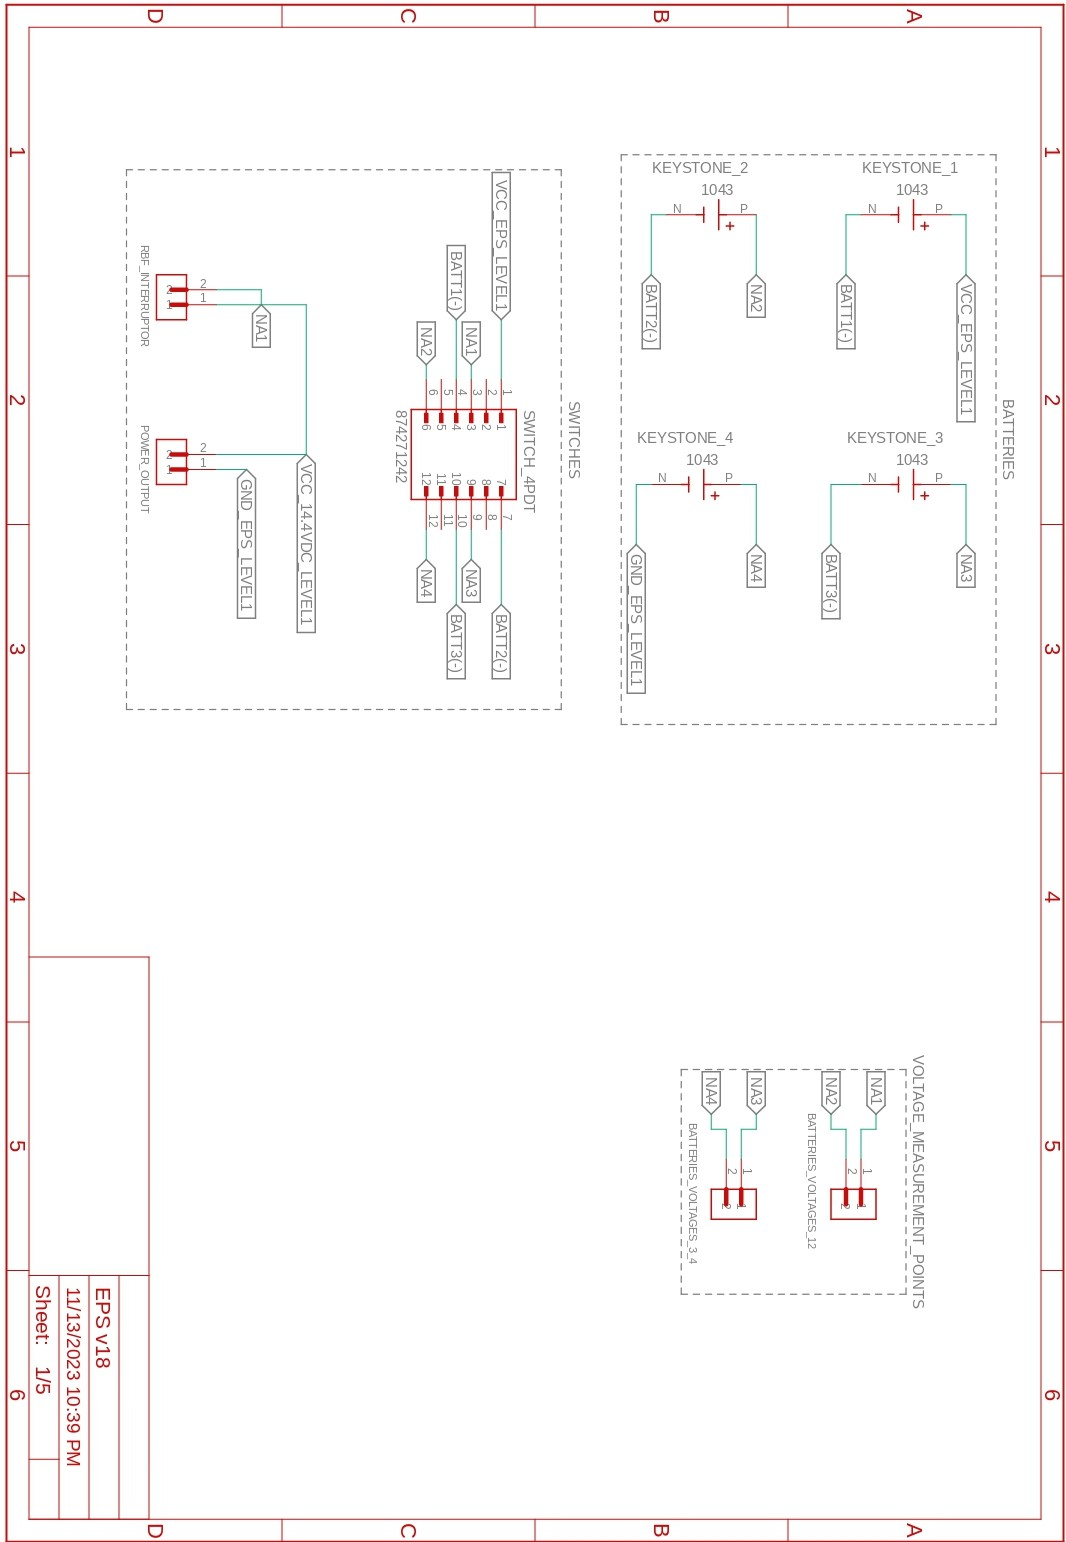
\includegraphics[width=0.6\textwidth, angle=90]{EPS_Sheets_page-0001.jpg} % Ajusta el tamaño y el ángulo según sea necesario
        \mycaption{Hoja 1 de esquemático del EPS}
        \label{fig:Esquematico1}
    \end{figure}
\end{frame}


%PAGINA 12

\begin{frame}
    \frametitle{Anexo 5}
    \framesubtitle{Integración del Sistema: Hardware}
    \begin{figure}[H]
        \centering
        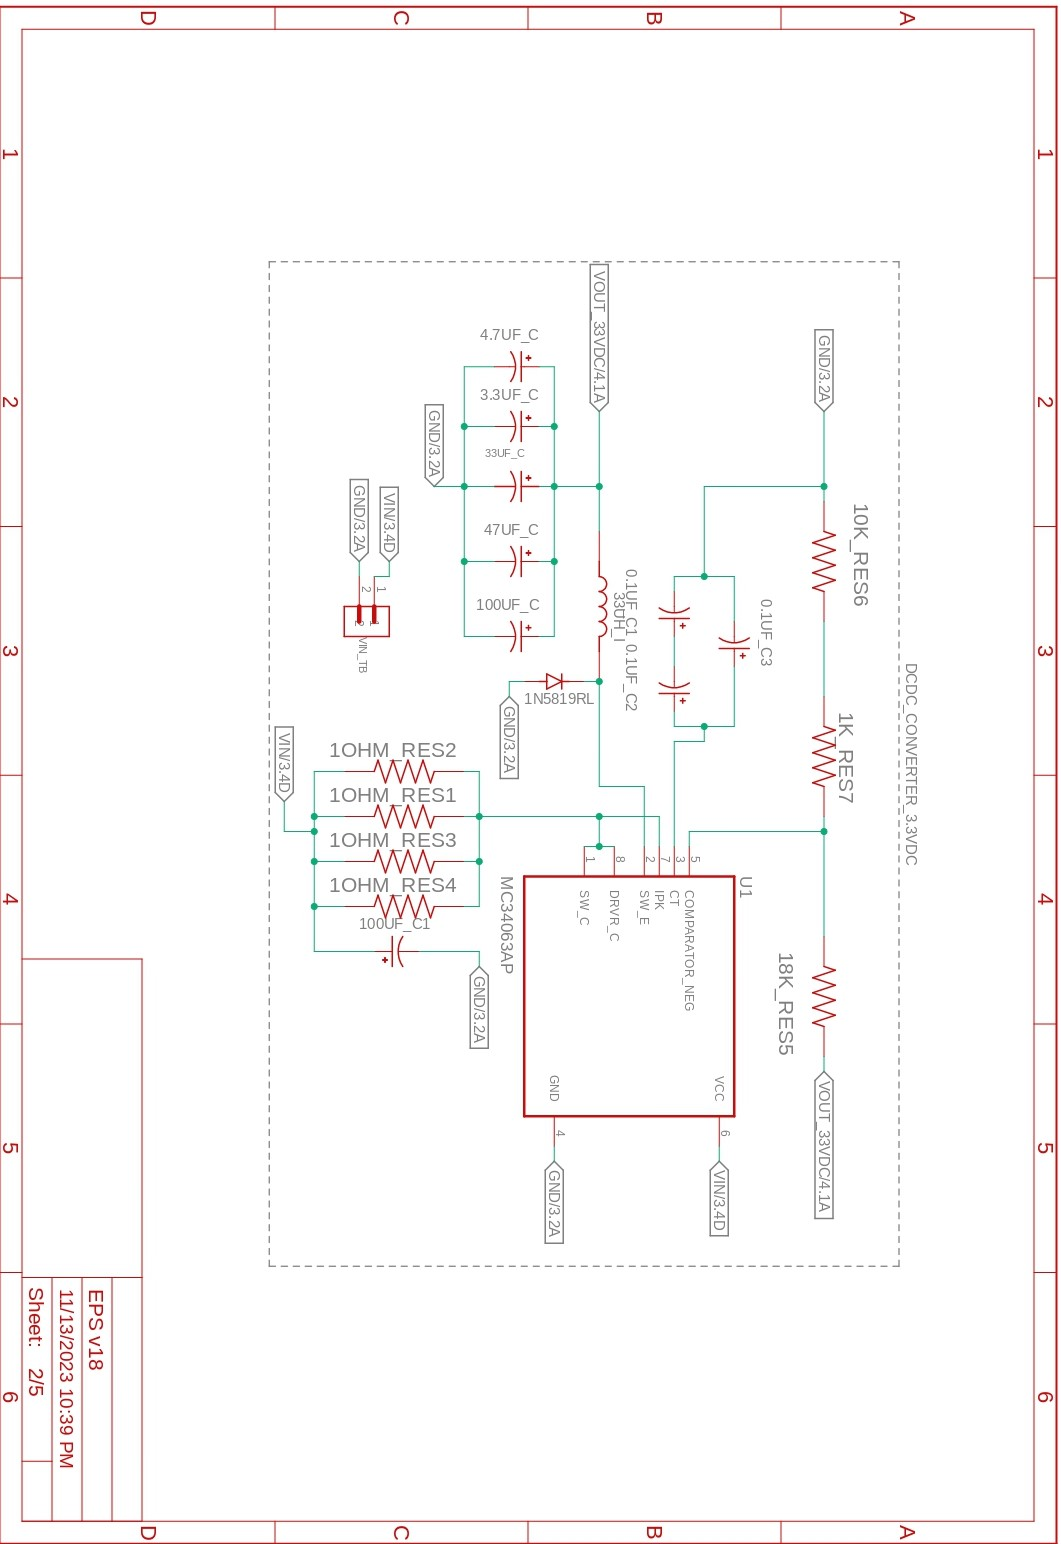
\includegraphics[width=0.6\textwidth, angle=90]{EPS_Sheets_page-0002.jpg} % Ajusta el tamaño según sea necesario
        \mycaption{Hoja 2 de esquemático del EPS}
        \label{fig:Esquematico2}
    \end{figure}
\end{frame}

%PAGINA 13

\begin{frame}
    \frametitle{Anexo 5}
    \framesubtitle{Integración del Sistema: Hardware}
    \begin{figure}[H]
        \centering
        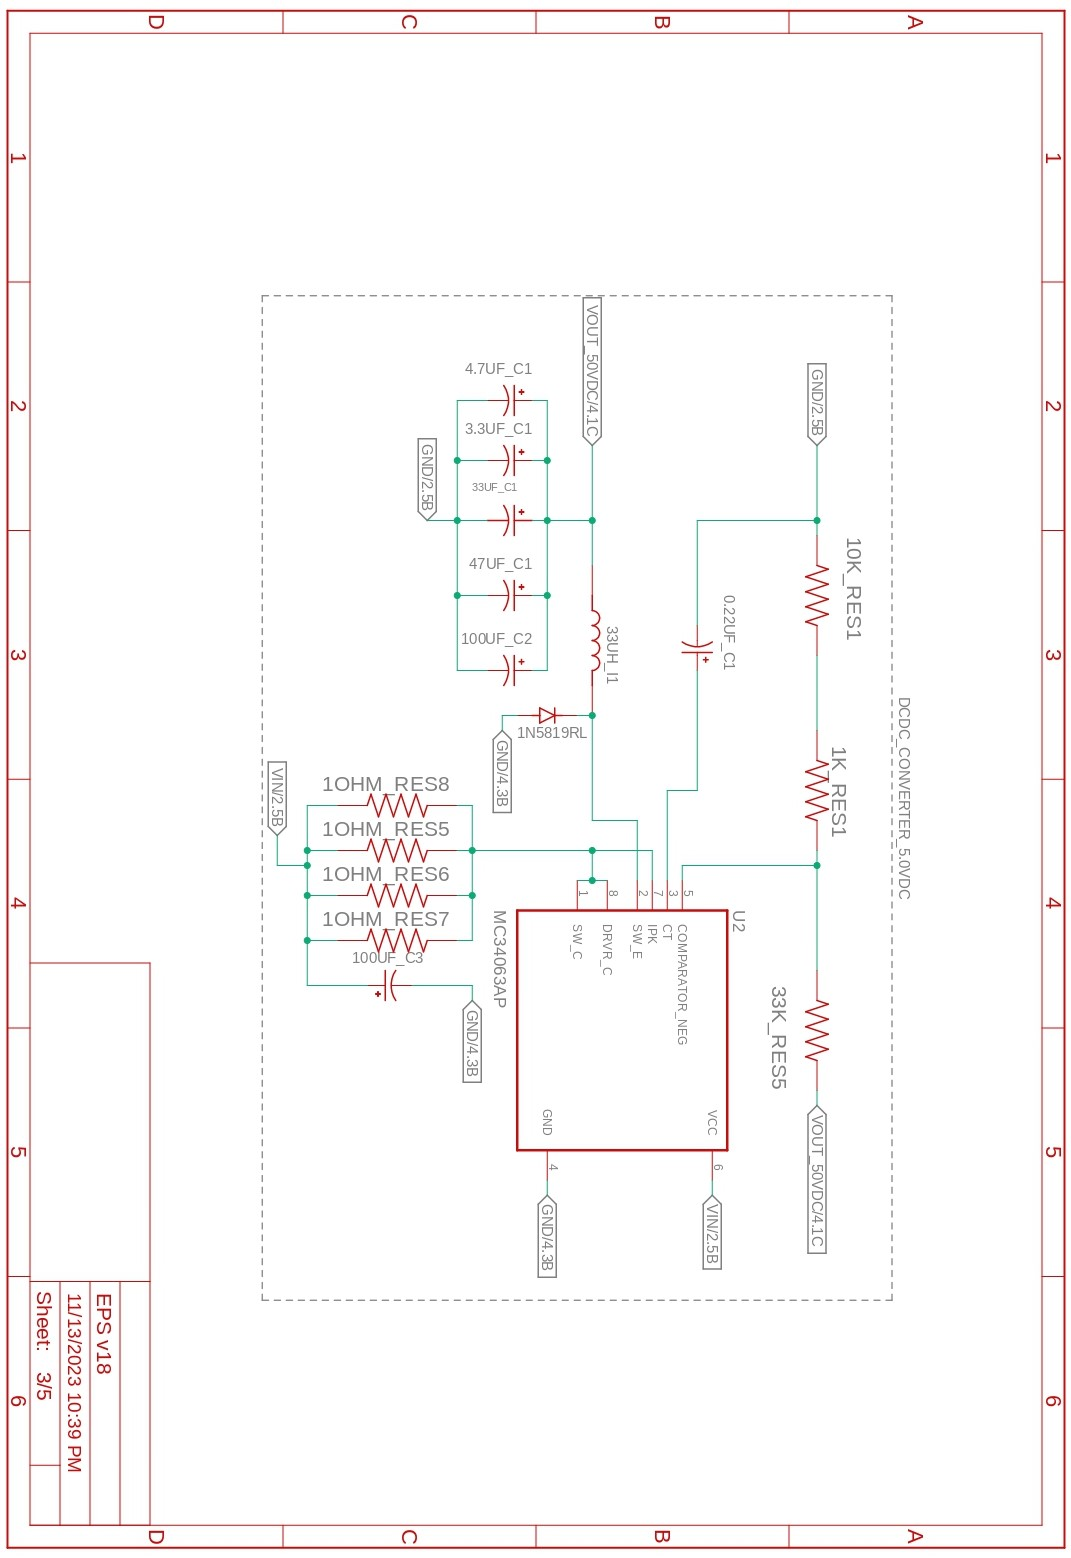
\includegraphics[width=0.6\textwidth, angle=90]{EPS_Sheets_page-0003.jpg} % Ajusta el tamaño según sea necesario
        \mycaption{Hoja 3 de esquemático del EPS}
        \label{fig:Esquematico4}
    \end{figure}
\end{frame}

%PAGINA 14

\begin{frame}
    \frametitle{Anexo 5}
    \framesubtitle{Integración del Sistema: Hardware}
    \begin{figure}[H]
        \centering
        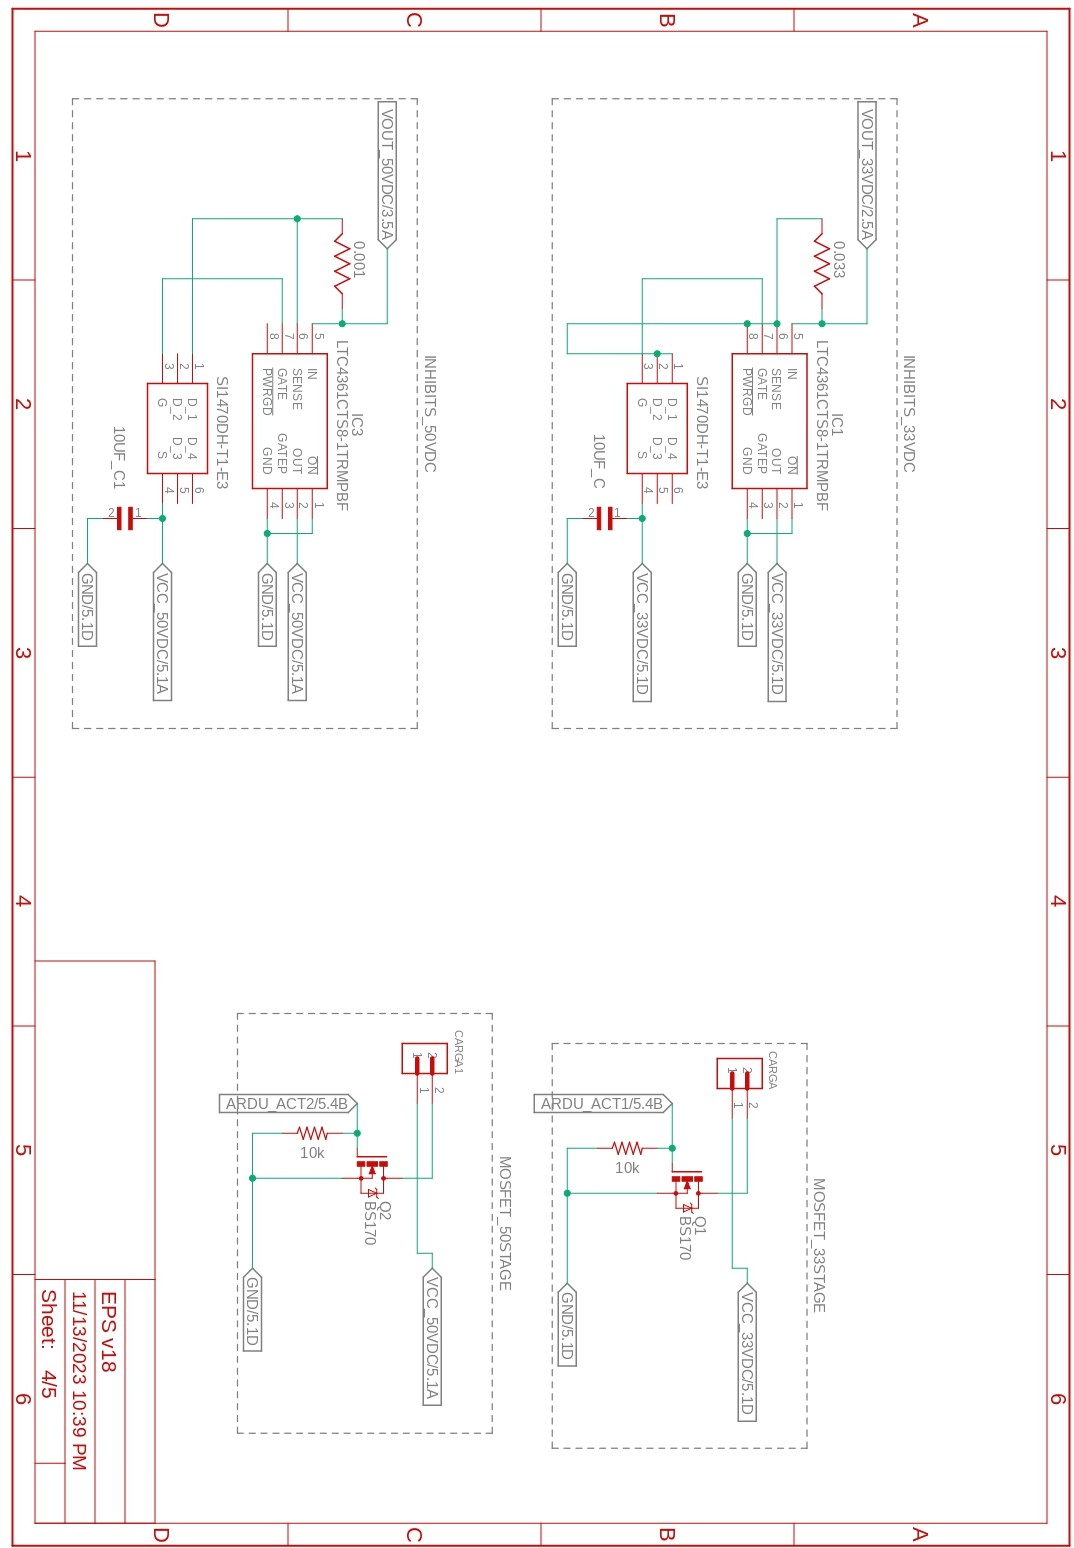
\includegraphics[width=0.6\textwidth, angle=90]{EPS_Sheets_page-0004.jpg} % Ajusta el tamaño según sea necesario
        \mycaption{Hoja 4 de esquemático del EPS}
        \label{fig:Esquematico4}
    \end{figure}
\end{frame}

%PAGINA 15

\begin{frame}
    \frametitle{Anexo 5}
    \framesubtitle{Integración del Sistema: Hardware}
    \begin{figure}[H]
        \centering
        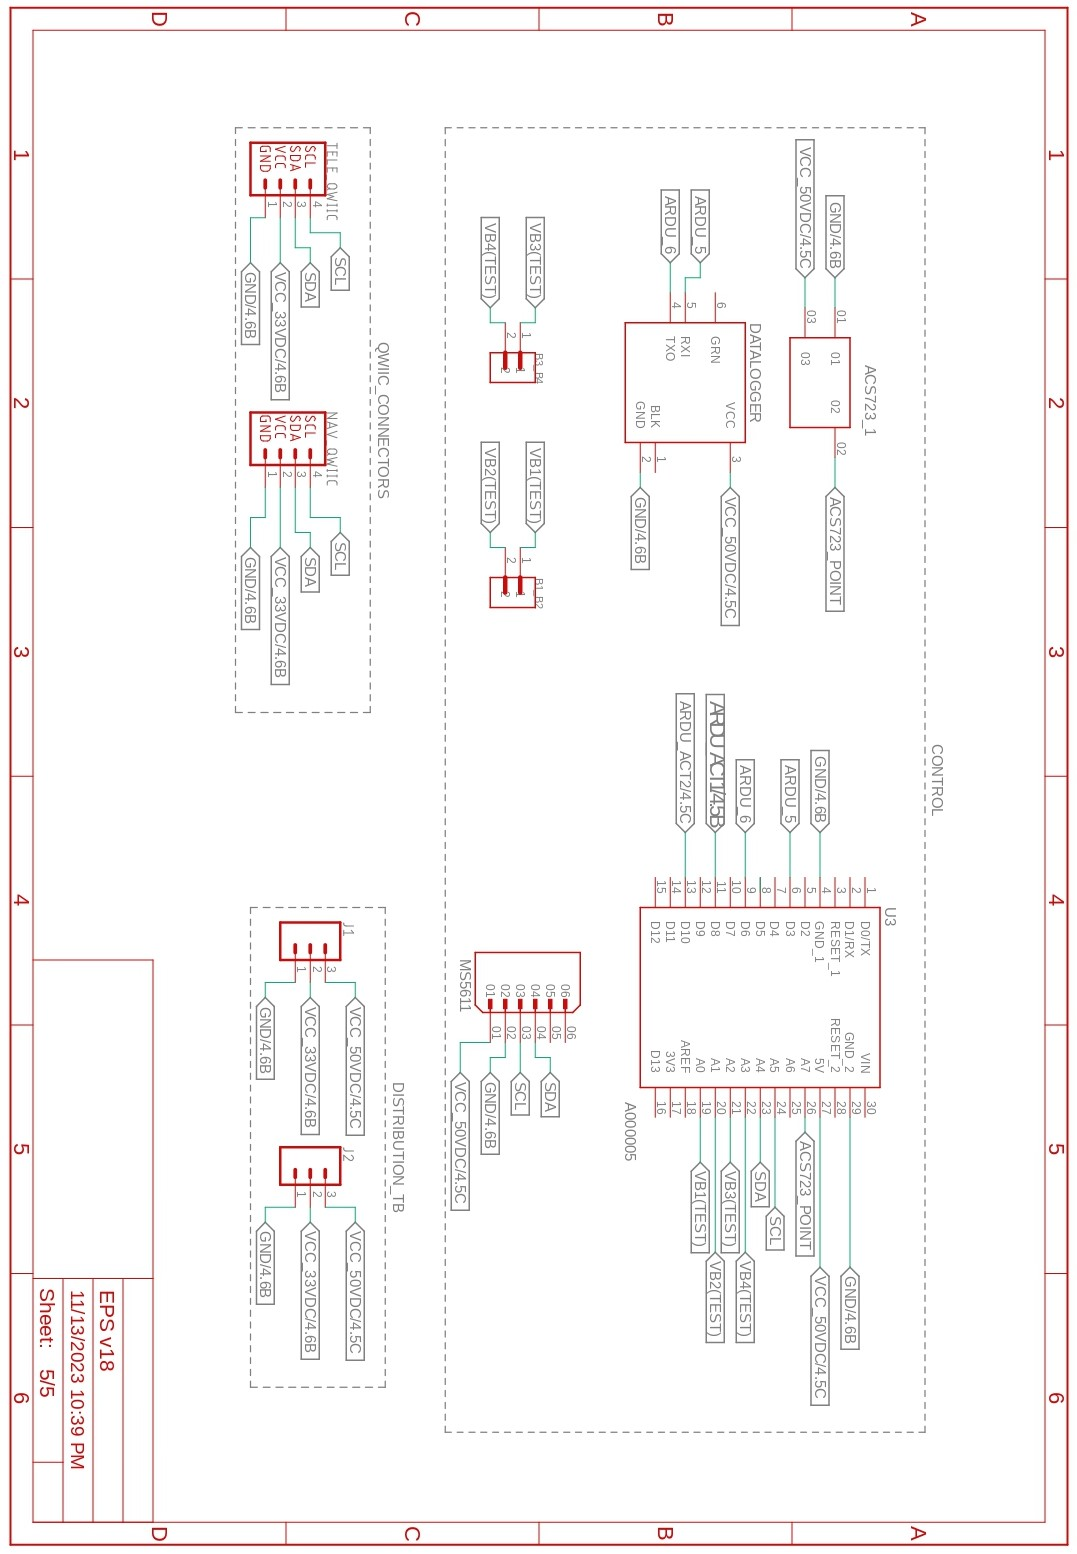
\includegraphics[width=0.6\textwidth, angle=90]{EPS_Sheets_page-0005.jpg} % Ajusta el tamaño según sea necesario
        \mycaption{Hoja 5 de esquemático del EPS}
        \label{fig:Esquematico5}
    \end{figure}
\end{frame}

%PAGINA 16

\begin{frame}
    \frametitle{Anexo 6}
    \framesubtitle{Contribuciones de la Tesis}
    \begin{itemize}
        \item Aplicación de Metodología de la NASA: Adaptación y aplicación en el diseño y desarrollo de un EPS para HAB.
        \item Desarrollo Integral del EPS: Incluye documentación detallada sobre desarrollo con software libre y electrónica COTS.
        \item Caracterización ambiental a lo largo de la trayectoria de un HAB: análisis del comportamiento de variables ambientales, como temperatura y presión, basado en datos provenientes de simulaciones de la trayectoria. Véase el Anexo B del documento de la Tesis.
    \end{itemize}
    
    
\end{frame}

%PAGINA 17

\begin{frame}
    \frametitle{Anexo 7}
    \framesubtitle{Trabajos Futuros}
    \begin{itemize}
        \item Cargador de baterías a bordo.
        \item Cámara de Vacío Térmico de Bajo Costo.
        \item Convertidor DC-DC para Arreglo de Baterías 1s4p.
        \item Diseño de Circuito de Descarga a Corriente Constante para Baterías de
        Iones de Litio.
    \end{itemize}
    
\end{frame}

%PAGINA 18

\begin{frame}
    \frametitle{Anexo 8}
    \framesubtitle{Presupuesto: EPS}
 
    \begin{table}[!ht]
        \centering
        \begin{tabular}{ll}
        \hline
            \textbf{\hfill Presupuesto de Compras \hfill} &  \\ \hline
            Local & \$64.59 \\ 
            Internacional & \$220.696 \\ 
            \hline
            Total & \$285.286 \\ 
        \hline
        \end{tabular}
        \caption{Resumen del Presupuesto de Compras}
        \label{tab:presupuesto}
    \end{table}
    
    
\end{frame}


\newpage

\section*{Bibliografía}
% Bibliografia
\printbibliography[heading=none]
\newpage

%--------- PREGUNTAS Y RESPUESTAS -----------

\end{document}
